\documentclass{seal_thesis}

% ---------------------- INSERT USED PACKAGES HERE ---------------------- 
\usepackage{xspace}
\usepackage{tabularx,ragged2e} 
\usepackage{anyfontsize}
\usepackage{amsmath}
\usepackage[table,xcdraw]{xcolor}
\usepackage[normalem]{ulem}
\useunder{\uline}{\ul}{}
\usepackage{url}

% === Per gli snippet =====================================
\lstset{
  backgroundcolor=\color{white},   % choose the background color; you must add \usepackage{color} or \usepackage{xcolor}
%  basicstyle=\footnotesize,        % the size of the fonts that are used for the code
  breakatwhitespace=false,         % sets if automatic breaks should only happen at whitespace
  breaklines=true,                 % sets automatic line breaking
  captionpos=n,                    % sets the caption-position to bottom
  deletekeywords={},			   % if you want to delete keywords from the given language
  escapeinside={\%*}{*)},          % if you want to add LaTeX within your code
  extendedchars=true,              % lets you use non-ASCII characters; for 8-bits encodings only, does not work with UTF-8
  frame=single,                    % adds a frame around the code
  keepspaces=true,                 % keeps spaces in text, useful for keeping indentation of code (possibly needs columns=flexible)
  language=java,                      % the language of the code
  morekeywords={},            	   % if you want to add more keywords to the set
  numbers=left,                    % where to put the line-numbers; possible values are (none, left, right)
  numbersep=5pt,                   % how far the line-numbers are from the code
  numberstyle=\tiny\color{gray}, % the style that is used for the line-numbers
  rulecolor=\color{black},         % if not set, the frame-color may be changed on line-breaks within not-black text (e.g. comments (green here))
  showspaces=false,                % show spaces everywhere adding particular underscores; it overrides 'showstringspaces'
  showstringspaces=false,          % underline spaces within strings only
  showtabs=false,                  % show tabs within strings adding particular underscores
  stepnumber=1,                    % the step between two line-numbers. If it's 1, each line will be numbered
  tabsize=2                       % sets default tabsize to 2 spaces
%  title=\lstname                   % show the filename of files included with \lstinputlisting; also try caption instead of title
}

% ---------------------- INSERT CUSTOMIZED COMMENTS HERE ---------------------- 
\newcommand{\toolname}{\textsc{TACL}}
\newcommand{\dynodroid}{\textsc{Dynodroid }}
\newcommand{\monkey}{\textsc{Monkey }}
\newcommand{\sapienz}{\textsc{Sapienz }}
\newcommand\RQ[1]{\textbf{RQ$_#1$}}
\newcommand{\SessionLauncher}{\textsc{SessionLauncher}}
\newcommand{\FDroidCrawler}{\textsc{FDroidCrawler}}
\newcommand{\AppTester}{\textsc{AppTester}}
\newcommand{\Config}{\textsc{ConfigurationManager}}
\newcommand{\Cmd}{\textsc{CmdExecutor}}
\newcommand{\Stream}{\textsc{StreamGobbler}}
\newcommand{\Extractor}{\textsc{CrashLogExtractor}}
\newcommand{\Crash}{\textsc{CrashLog}}
\newcommand{\Lucene}{\textsc{LuceneTokenizer}}
\newcommand{\TFIDF}{\textsc{TFIDFCalculator}}
\newcommand{\Oracle}{\textsc{Oracle}}
\newcommand{\Review}{\textsc{Review}}
\newcommand{\ReviewC}{\textsc{ReviewCollector}}


% ---------------------- HERE STARTS THE THESIS BODY ---------------------- 
\thesisType{Bachelor Thesis}
\date{\today}
\title{GUI usability and testing of mobile applications}
\subtitle{Example subtitle}
\author{Lucas Pelloni}
\home{18.03.1993, Zurich} % Geburtsort
\country{Switzerland}
\legi{13-722-038}
\prof{Prof. Dr. Harald C. Gall}
\assistent{Dr. Sebastiano Panichella \\ Giovanni Grano (PhD student)}
\email{lucas.pelloni@uzh.ch}
%\url{https://github.com/lucaspelloni2/BA\_PROJ}
\begindate{08.01.2017}
\enddate{08.07.2017}

\begin{document}
\maketitle



\frontmatter


\thispagestyle{empty}

\begin{flushright}
\vspace*{3cm}
  {\Large \textit{{``Program testing can be used to show the presence of bugs, but never to show their absence.``}
  \\ \vspace{1cm} Edsger W. Dijkstra}}\\
\end{flushright}

\begin{acknowledgements}
The experience I lived with the implementation and subsequently the writing of my bachelor thesis was undoubtedly one of the most rewarding academic experiences of my life until now. During these six months, I learned to know more in-depth the programming world, appreciating more and more its challenges and its beauties.
However, the realization of my thesis would not have been possible without the help of few people. First, I would like to thank all those people who have contributed directly to the realization of my bachelor thesis. After that, those who indirectly allowed me to reach such an important goal of my life: my bachelor's degree.

First of all, I would like to express my deepest gratitude to my thesis advisor, Giovanni Grano. I would like to thank him for the patience he has shown during the past six months, for its guidance and support, for its constructive criticism and for having always encouraged me to achieve my best. I think one of the best things of my thesis was that he always allowed me to experiment and to be creative with the assigned tasks. I could  "bang my head" against the new challenges and this helped me to find the right solutions.
The final result of my thesis would not have been possible without his help. 
I would like to offer special thanks to Dr. Sebastiano Panichella for believing in me from the beginning and for giving me such a high-level thesis. Thanks for allowing me to discover a branch of computer science that I did not know so in detail before. 
I thank also my two computer science schoolmates, Ile and Erion, who helped me a lot with their knowledge about android mobile devices.
Finally, I would like to thank Professor Gall for giving me the opportunity to work together with the Software Evolution \& Architecture Lab at the University of Zurich, allowing me to use the most state-of-the-art infrastructures and technologies for my thesis. 

I would like to spend also some words for those people, who support me during the whole bachelor degree. 
%and I could explore it in a more practical way.
\end{acknowledgements}

\begin{abstract}
\end{abstract}

\begin{zusammenfassung}
\end{zusammenfassung}

\tableofcontents
\listoffigures
\listoftables
\lstlistoflistings

\mainmatter
\chapter{Introduction}
\label{sec:intro}
% !TEX root =  ./lucas_thesis.tex
%------------------------- THESIS OVERVIEW ------------------------
\label{chapter:intro}
This thesis is placed in the context of mobile automated testing. In particular, we aim to shed some initial lights into the possibility to integrate user feedback into such process, in order to increase its efficiency and efficacy.
The first chapter of this work gives an overview about the context in which the thesis is placed, as well as the motivations that led to such thesis. There follows a brief introduction about mobile testing, its limitations and challenges. At the end, we disclose the research questions leading our investigations. 
The remainder of this thesis is organized as follows: 

Chapter \ref{chapter:related} presents the recent literature in two areas of interest for this work, \ie automated mobile testing and the exploiting of mobile stores mining in order to facilitate the software maintenance activities.

Chapter \ref{chapter:approach} describes the approach we developed in order to investigate our main goal.

Chapter \ref{chapter:tool} presents \toolname, a tool that firstly relies on \monkey and \sapienz in order to test a set of Android applications, collecting crash logs (\ie stack traces). Secondly, exploiting classic Information Retrieval (IR) techniques, the tool is able to cluster the logs that refer to the same bugs. Finally, it relies on a novel approach for linking such clusters of crash logs with the users reviews that refer to the bug revealed by them. 
%The tool enables developers to link natural language contained inside user feedbacks and pieces of source code, such as names of classes, methods, functions, etc. 

Chapter \ref{chapter:results} describes the empirical study we conducted in order to evaluate the aforementioned approach on a set of 3 mobile apps (available on \textit{FDroid \footnote{\url{https://f-droid.org}}}) with their correspondent reviews crawled from the Google Play Store\footnote{\url{https://play.google.com/}}. 

Finally, Chapter \ref{chapter:conclusion} closes the main body of the thesis drawing the necessary conclusions and spreading the main ideas for future contributions.


%------------------------- CONTEXT: TESTING IN GENERAL -------------------
\section{Context}
Testing is the action of inspecting the behavior of a program, with the intention of finding anomalies or errors \cite{testing}.
The goal behind software testing is to exercise the system under test (SUT) in order to hopefully reveal as many bugs as possible. In order to do that, it aims to reach the highest \textit{test coverage} with the smallest number of \textit{test cases}. A test case can be viewed as a set of program inputs, each of them gets associated with an expected result (\ie \textit{oracle}) when they are executed. 

Nowadays, software testing is widely recognized as an essential part of any software development process, presenting however an extremely expensive activity. Indeed, testing all combinations of all possible input values classes for an application \cite{glinz} requires a lot of workforce and it is almost always unthinkable to reach a testing-coverage of 100\%. 
Furthermore, testing is often performed under time and budget constraints \cite{grano} and complex applications might have a very large number of potential test scenarios, many of which could be really difficult to predict. Indeed, \textit{Dijkstra} \cite{dijkstra} observed that testing a software does not imply a demonstration of the right behaviour of the program, but it only aims to demonstrate the presence of faults, not their absence. 
%But then, why try to test a program even knowing that a full coverage (and so a complete validation of the software) cannot be reached? Well, the answer is quite simple. 
So, deeply testing a SUT increases the probability that this software will behave as expected also in the untested cases \cite{glinz}. 

In general, there are four testing levels a tester should perform in order to investigate the behaviour of a traditional software: 
\begin{enumerate}
\item Unit testing; 
\item Integration testing; 
\item System testing; 
\item Acceptance testing.
\end{enumerate}

With \textit{unit testing}, the application components are viewed and split into  individual \textit{units} of source code, which are normally functions or small methods. Intuitively, one can view a unit as the smallest testable part of an application. This kind of testing is usually associated with a \textit{white-box} approach. \textit{Integration testing} is the activity of finding faults after testing the previous individually tested units combined and tested as a group together. \textit{System testing} is conducted on a complete, integrated system to evaluate the compliance with its requirements. It can be imagined as the last checkpoint before the end customer. Instead, \textit{acceptance testing} (or \textit{customer testing}) is the last level of the testing process, which states whether the application meets the user needs and whether the implemented system works for the user. This kind of testing is usually associated with a \textit{black-box} approach. 
\\
These mentioned testing levels shall be sequentially executed and are driven by two testing methodologies \cite{white-box, black-box}: 
\begin{itemize}
\item black-box testing;
\item white-box testing.
\end{itemize} 
With \textit{black-box} testing (also called functional testing) the tester does not have any prior knowledge of the internal structure of the SUT. He tests only the functionalities provided by the software without any access to the source code. Typically, when performing a black box test, a tester interacts with the system's user interface by providing inputs, examining the compliance of the output with the oracles. 
On the other hand, with \textit{white-box} testing (also \textit{glass testing} or \textit{open box testing}), the test cases are extrapolated from the internal software's structure \cite{grano}. Indeed, the tester writes the test cases that reflect paths through the code, with the aim usually to maximize a coverage criterion. 
At the end, those techniques aim to generate a \textit{test suite} composed by a set of \textit{test cases}, \ie a set of conditions under which a tester will determine whether a software system is working as it was described by its original specification.

As previously explained, testing can be done through different approaches, methodologies and level of details. However, the common goal behind the testing remains the same, i.e. generating the smaller test suiteable to reveal the largest number of failures, in order to increase the reliability of the system \cite{grano}. 
Nevertheless, the process of finding the correct test scenarios, generating the consequential data inputs, executing and finally reporting the results, comparing them to the previously written specifications, might be time-consuming and cost-intensive. In fact, testing costs have been estimated at being at least half of the entire development cost \cite{Beizer:1990:STT:79060}. For this reason, it is necessary to reduce such costs automatizing the various processes occurring in testing, trying to improve the effectiveness of the whole process. In such described scenario, for instance, a remarkable example is the application of Search-Based approaches that have been successfully exploited in the last years in order to automate the test data generation \cite{Harman_et_al_2015}.§

\section{Motivation}
%------------- PASSAGGIO DAL TESTING TRADIZIONALE AL MOBILE -------------
In the last years, we have witnessed a huge growth in the usage of mobile software, due to the advent of the \textit{mobile age}. Indeed, nowadays, application running on mobile devices are becoming so widely adopted, so that they have represented a remarkable revolution in the IT sector. In fact, in three years, over 300,000 mobile applications have been developed \cite{muccini}, 149 billions downloaded only in 2016 \cite{statista} and 12 million mobile app developers (expected to reach up 14 million in 2020) maintaining them \cite{DevRelate}. 

Because of the importance of the mobile development field nowadays, developers aim to sustain the competition in acquiring and retaining users increasing the quality of their application. 
Since testing plays a crucial role in achieving such quality, several approaches for automated mobile testing have been recently developed. This because, mobile applications differ from traditional software and so there is also a need for developing new ad-hoc testing techniques. 
In fact, mobile applications are structured around Graphical User Interface (GUI) events and activities, thus exposing them to new kinds of bugs and leading to a higher defect density compared to traditional desktop and server applications \cite{Hu:2011:AGT:1982595.1982612}. Furthermore, they are context-aware \cite{muccini}. 
This means that each mobile application is aware of the environment in which it is running and exposes a different behavior according to its current context. This has some implications for the testing, because a test case running on a specific context may lead to different results. In fact, bugs related to contextual inputs are quite frequent \cite{muccini}. 

For this reason, mobile applications require new specialized and different testing techniques in order to ensure their reliability \cite{muccini}. Being mobile applications event-based systems used through UI interaction, the GUI testing needs to have a prominent role in app testing. In particular, in this kind of testing, each test case is designed and run in the form of sequences of GUI interaction events, with the aim to state whether an application meets its written requirements. 

% ------------- LE SFIDE DEL MOBILE TESTING E AUTOMATED GUI TESTING -----------------
As traditional testing, GUI testing can be performed either manual or automatic. However, a manual approach would require a lot of programming and may be time-consuming. 
For this purpose, with the aim to support developers in building high-quality applications, the research community has recently developed novel techniques and tools to automate their testing process \cite{sapienz, dynodroid ,muccini,Hu:2011:AGT:1982595.1982612}. 
%The most famous automated GUI testing tools and their properties are discussed in the chapter \textit{Related Work}. \\
These techniques consist of automatically creating test cases through the generation of UI and system events, which are transmitted to the application under test, with the aim to cause some crashes. Afterwards, if an exception occurred, these tools usually save in log files the correspondent stack traces, along with the sequence of events that led to the exceptions \cite{muccini}. 
However, despite a strong evidence for automated testing approaches in verifying GUI application and revealing bugs, these state-of-art tools cannot always achieve a high code coverage \cite{Nagappan2015}. 
One reason is that current approaches are not suited for generating inputs that require human intelligence (e.g. \textit{"inputs to text boxes that expect valid passwords, or playing and winning a game with a strategy"}) \cite{dynodroid}. This inability to replicate the human behaviour, often leaving feature and crash bugs undetected until they are encountered by the users.
Furthermore, current solutions generate redundant/random causing incredibly long sequences of events needed to replicate a crash, while most of such inputs could be avoided. 
In addition, the crash reports that they generate usually lack of contextual information and are difficult to understand and analyze \cite{Chen, Joorabchi}. 
For such reasons, sometimes a time-consuming manual intervention may be needed for testing appropriately an application \cite{Nagappan2015}. 

% ------------- REVIEWS PER AIUTARE GLI SVILUPPATORI NELLA FASE DI TESTING -----------------
Despite these limitations and challenges, the mobile developing environment has the huge advantage, compared to the traditional one, of having a huge amount of information available from mobile stores, which have been introduced as a new selling paradigm for mobile applications. Indeed, the exponential growth of the mobile stores offers an enormous amount of information and feedbacks from users that researchers and partitioner can use to develop better applications. In fact, these users feedback are playing more and more a paramount role in the development and maintenance of mobile applications. Indeed, recent research focused on how such knowledge might be successfully exploited (Section \ref{section:review_usage}). 
We argue that also the GUI testing could take profit in some way of this information. That is why, in this thesis work we shed some initial lights into the integration of feedbacks extracted from user reviews in the automated testing for mobile applications.
In detail, we hypothesize that such integration can be exploited to overcome the aforementioned limitations of state-of-the-art tools for automated testing of mobile apps in the following ways \cite{cristal}: 
\begin{enumerate}
\item it can complement the capabilities of automated testing tools, by identifying bugs that they cannot reveal; 
\item it can facilitate the diagnosis and reproducibility of bugs (or crashes), since user reviews often describe the actions that led to a failure; 
\item it can be used to prioritize bug resolution activities based on the users' requests, possibly helping developers in increasing the ratings of their apps.
\end{enumerate} 
In particular, in this work we investigated this first point by developing an approach able to link the user reviews with the stack traces that refer to the same bug. Furthermore, we conducted a preliminary study to understand how complementary are the two sources of information and in particular whether we can use the reviews to identify some problems that the tools miss. 

\section{Motivation Example}
Following, we provide a concrete example of how we plan to compare and analyse the two sources of information: user reviews and reports generated by automated mobile applications testing tools. Given app reviews, we first plan to automatically select the ones describing crashes and bugs in features or in UI elements.
%\textit{Feature \& UI Bugs} and \textit{Crashes}. 
A good example of useful review is the following: 
\smallbreak
\emph{\small``Barely works I only installed this for the android sharing function but it usually loads a white screen when I try to use this feature. It's no better than using a browser to view Facebook otherwise.''}. 
\smallbreak
The user here complains about the app sharing function that shows a white screen when activated. A report generated by one of available automated testing tools, \textsc{Sapienz} \cite{sapienz}, includes the stack trace below, where \sapienz is able to find a \texttt{NullPointerException} while exercising the sharing functionality. 
\smallbreak
\begin{lstlisting}[basicstyle=\fontsize{5.5}{8}\ttfamily]
java.lang.NullPointerException
  at com.danvelazco.fbwrapper.activity.BaseFacebookWebViewActivity.shareCurrentPage(BaseFacebookWebViewActivity.java:418)
  at com.danvelazco.fbwrapper.FbWrapper.access$700(FbWrapper.java:26)
  at com.danvelazco.fbwrapper.FbWrapper$MenuDrawerButtonListener.onClick(FbWrapper.java:376)
  at android.view.View.performClick(View.java:4438)
  at android.view.View.onKeyUp(View.java:8241)
  ....
  ....
  at com.android.internal.os.ZygoteInit.main(ZygoteInit.java:611)
  at dalvik.system.NativeStart.main(Native Method)
\end{lstlisting}
\smallbreak
So, the aim behind this thesis is to investigate the complementarity between the user reviews and the crash reports generated by the automated state-of-art tools described in Section \ref{sec:tools}.
The preliminary step into this analysis it to implement a linking procedure of the two sources of information. We argue that this approach can be fruitfully used to support developers in determining which bugs should be addressed first, prioritizing the arising failures. It is worth noticing that such prioritization is directly guided by the users feedback with the aim to maximize their satisfaction and consequentially, the app rating.
We argue that this investigation might improve the automated testing process and might help other developers in validating their mobile applications, using \toolname, the implemented tool described in the Chapter \ref{chapter:tool}.

\section{Research questions}
\label{section:rqs}
In this thesis, we conduct a preliminary study to investigate the first and most important point from the previous list, \ie \textit{the complementarity between user feedback and the outcomes of automated testing tools}. This research represents a first fundamental step toward the integration of user feedback into the testing process of mobile apps. Thus, we conducted my thesis aiming to answer the following research questions:

\begin{itemize}
	\item \RQ{1}: \textit{Which are the most important tools for automatic testing of Android applications?} %I want to investigate 
	\item \RQ{2}: \textit{To what extent can we link the defects arose from automated testing tools with user reviews?}  
%	\item \RQ{3}: \textit{What kind of defects are detected by state-of-art tools proposed for GUI testing? How these defects are effectively perceived by users?} 
	\item \RQ{3}: \textit{How complementary are the two source of information? Can we leverage on both of them to increase the effectiveness of the testing process?}
\end{itemize}
The first research question is merely represented by a literature overview to identify which are the state-of-art tools in automated Android testing. To answer such question we presented the main research in this field in Chapter \ref{sec:related}, giving an accurate overview of testing tools in general, their pros and cons and their different exploration strategies. 

To answer the \RQ{2}, we implement a linking procedure which relies on Information Retrieval (IR) techniques and uses an experimental-based threshold in order to state whether a review refers to a specific stack trace. We described the implemented approach in Chapter \ref{chapter:approach}, discussing its precision in Chapter \ref{chapter:results}.
Finally, for our last research question we relied on the aforementioned implemented linking technique to understand and identify whether particular kind of bugs cannot be revealed by current testing tools but can be observed in user reviews (and vice versa). Again, we describe the achieved results in Chapter \ref{chapter:results}.

\chapter{Related Work}
\label{sec:related}
% !TEX root =  ./lucas_thesis.tex
\label{chapter:related}
In the following two sections, I summarize the main related works on \textit{automated testing tools for Android apps} and on \textit{the broadly usage of user reviews from app store in Software maintenance activities}. 
An overview of the recent research in the field can be found in the survey by Martin \etal \cite{Martin:tse2017}. 
\section{Automated tools for Android Testing}
\label{sec:tools}
%Unlike traditional software, mobile applications are mainly exercised by user inputs. \\ 
%In the mobile world, an extremely valid approach to ensure the reliability of these applications is the GUI\footnote{Graphical User Interface} Testing. \\ 
%In particular, in this kind of testing, each test case is designed and run in the form of sequences of GUI interaction events.  \\
Depending on their exploration strategy, there are in general three approaches for creating a generation of user inputs on a mobile device \cite{dynodroid, areWeThereYet}: \textit{random testing} \cite{dynodroid, monkey}, \textit{systematic testing} \cite{evodroid} and \textit{model-based testing} \cite{mobiguitar, swift, mining}. 
\subsubsection{Fuzz testing}
When test automation does occur, it typically relies on Google's Android \monkey command-line \cite{monkey}. Since it comes directly integrated in Android Studio, the standard IDE for Android Development, it is regarded as the current state-of-practice \cite{evodroid}.
This tool simply generates, for the specified Android applications, pseudo-random streams of user events into the system, with the goal to stress the \textit{AUT\footnote{Application Under Test}} \cite{monkey}.  
The effort required for using \monkey is very low \cite{areWeThereYet}. Users have to specify in the command-line the type and the number of the UI events they want to generate and in addition they can establish the verbosity level of the \monkey log. 
The set of possible \monkey parameters can be found in the official \textit{User Guide} for \monkey on \cite{monkey}. \\
The kind of testing implemented by \monkey follows a black-box approach. 
Despite the robustness, the user friendliness \cite{areWeThereYet, dynodroid} and the capacity to find out new bugs outside the stated scenarios  \cite{monkey_2}, this tool may be inefficient if the \textit{AUT} would require some human intelligence (\textit{e.g.} a login field) for providing sensible inputs \cite{dynodroid}. \\
For this reason, \monkey may cause highly redundant and senseless user events. Even though it would find out a new bug for a given app, the steps for reproducing it may be very difficult to follow, due also to the randomness in the testing strategy implemented by it \cite{monkey_2}. 


\textbf{Dynodroid} \cite{dynodroid} is also a random-based testing approach. However, this tool has been discovered being more efficient than \monkey in the exploration process  \cite{areWeThereYet}. \\
One of the reasons behind a better efficacy has been that \dynodroid is able to generate both \textit{UI inputs} and \textit{system events} (unlike \monkey, which can only generate UI events) \cite{areWeThereYet}. \\  
Indeed, \dynodroid can simulate an incoming SMS message on a mobile device, a notification of another app or an request of use for available wifi networks in the neighborhood \cite{dynodroid}. All these events represent \textit{non-UI events} and they are often unpredictable and therefore difficult to simulate in a suitable context. 
\dynodroid views the AUT as an event-driven program and follows a cyclical mechanism, also known as the \textit{observe-select-execute} cycle \cite{dynodroid}. First of all, it \textit{observes} which events are relevant to the AUT in the current state, grouping they together (an event must be considered relevant if it triggers a part of code which is part of the AUT). After that, it \textit{selects} one of the previously observed events with a randomized algorithm \cite{dynodroid, areWeThereYet} and finally \textit{executes} it. After the execution of that event the AUT reaches a new state and the cycle again stars again. \\
Another advantage of \dynodroid compared to \monkey is that it allows users to interact in the testing process providing UI inputs. In doing so, \dynodroid is able to exploit the benefits of combining automated with manual testing \cite{dynodroid}.

\subsubsection{Systematic testing}
The tools using a systematic explorations strategy rely on more sophisticated techniques, such as symbolic execution and evolutionary algorithms \cite{areWeThereYet}. 


\sapienz \cite{sapienz} introduced a new Pareto multi-objective search-based technique (the first one to Android testing) to simultaneously maximize coverage and fault revelation, while minimizing the sequence lengths. Its approach combines the above mentioned random-based techniques with a new systematic exploration. \sapienz starts its work-flow by instrumenting the AUT, which can be achieved using a \textit{white-box} approach, whether the source code is available. Otherwise the "instrumenting-process" follows a \textit{black-box} approach whether only the APK\footnote{Android Package Kit, extension used by Android OS for installing a mobile app on an android device} is given.  
Afterwards, \sapienz extracts string constants after an accurate analysis of the APK. These strings are used as inputs for inserting realistic strings into the AUT, which has been demonstrated to improve the testing efficiency \cite{sapienz}. After that, UI events are generated and executed by an internal component called \textit{MotifCore}. 
This component, as highlighted before, combines random-based testing approaches with systematic exploration strategies. When it gets invoked, it initialises an \textit{initial population} via \textit{MotifCore's Test Generator} and starts the genetic evolution process. 
During this process, another component called \textit{Test Replayer} manages genetic individuals during the evaluation process of the individual fitness. After that, the individual test cases are translated into Android events by the \textit{Gene Interpreter}, which is in charge of communicate with the mobile device. 
Another component called \textit{States Logger} checks whether the tests cases find some faults and produces statistics for another component, called \textit{Fitness Extractor}, which compute the fitness. \\
Finally, reports containing data about testing results, such as code coverage, stack traces and "steps for reproducing the faults" are generated and stored at the end of the process.  


The experiment results published on \cite{sapienz} show that \sapienz is an out-performer in the automated mobile testing area. The table below compares the above mentioned tools \monkey and \dynodroid with \sapienz, illustrating the strength of the \sapienz's approach. 

\begin{table}[tb]
\centering
\caption{Statistics on found crashes from the \sapienz experiment published on \cite{sapienz}}
\label{sapienz experiment results}
\begin{tabular}{|c|c|c|c|l}
\cline{1-4}
\textbf{App crashes} & \textbf{Monkey} & \textbf{Dynodroid} & \textbf{Sapienz} &  \\ \cline{1-4}
Nr. App crashes      & 24              & 13                 & 41               &  \\ \cline{1-4}
Nr. Unique crashes   & 41              & 13                 & 104              &  \\ \cline{1-4}
Nr. Total crashes    & 1'196           & 125                & 6'866             &  \\ \cline{1-4}
\end{tabular}
\end{table}
As represented in the table above, \sapienz found from a set of 68 benchmark apps, 104 unique crashes (while \monkey 41 and \dynodroid 13).

\subsubsection{Model-based testing}
Model-based tools for testing Android applications are quite popular \cite{sapienz}. Most of these tools \cite{mobiguitar, mining, guiripper,swift} generate UI events from models, which are either manually designed or created from XML configuration files \cite{sapienz}. \\
For example, \textit{SwiftHand} \cite{swift} uses a machine learning algorithm to learn a model of the current \textit{AUT}. This final state machine model \cite{areWeThereYet} generates UI events and due their execution the app reaches new unexplored states. After that, it exploits the execution of these events to adapt and refine the model \cite{swift}. \textit{SwiftHand}, in a similar way to \monkey generates only touching and scrolling UI events and is not able to generate System events \cite{areWeThereYet}.

% TODO: allargare questa sezione 
\section{Usage of users reviews in Software maintenance activities}
\label{section:review_usage}
The concept of app store mining was first introduced by \textit{Harman} \etal
\cite{appstoremining}. In this context, many researchers focused on the analysis of user reviews to support the maintenance and evolution of mobile applications \cite{Martin:tse2017}.
Pagano \etal \cite{pagano} empirically analyzed the feedback content and their impact on the user community, while Khalid \etal \cite{Khalid:2015:IEEE} conducted a study on iOS apps discovering 12 types of user complaints posted in reviews. Several approaches have been proposed with the aim to classify useful reviews.
\textsc{AR-Miner} \cite{Chen} represents the first  approach proposed in the literature able to discern  informative reviews. 
In this direction, in a recent work Panichella \etal introduced a tool called \textsc{surf} (Summarizer of User Reviews Feedback), that is able to analyse the useful informations contained in app reviews and to performs a systematic summarisation of thousands of user reviews through the generation of an interactive agenda of recommended software changes \cite{DBLP:conf/sigsoft/SorboPASVCG16}. \\
Finally, Palomba \etal \cite{Palomba2017} proposed \textsc{ChangeAdvisor}, a tool able to suggest the source code artifacts to maintain according to user feedback.

%------------------ WHY SAPIENZ AND MONKEY ----------------
\label{sec:choicetool}
\section{Choice and motivation for the used automated testing tools}
For the implementation of \toolname, we have chosen to use the following two automated testing tools: 
\begin{itemize}
\item \monkey
\item \sapienz
\end{itemize}
The selection of \monkey is justified by the fact that (i) \monkey represents the current state-of-practice in the field of automated mobile testing \cite{evodroid} and therefore is well supported and documented by the community, (ii) the effort for using it is very low \cite{areWeThereYet}  and (iii) being it a command-line tool, it can easily be combined with the terminal and so be launched by and integrated into an external tool which provides and supports command-line functions.  

The aim of selecting \sapienz is driven by the fact that (i) \sapienz has been found to be (based on the experimental results presented on \cite{sapienz}) an out-performer in the automated mobile testing area. Indeed its approach has been discovered to be much more reliable and high-performing compared to other testing strategies such as those of \monkey or \textsc{Dynodroid}. (ii) The source code of \sapienz is readily accessible on \textit{GitHub} and therefore the whole source code can be integrated into another tool (iii) \sapienz can also be started using some command-lines. 












\chapter{Approach}
\label{sec:approach}
\label{chapter:approach}
In this work, we aim to build an approach able to (i) automatically test Android applications with modern state-of-art tools, (ii) automatically collect the arose errors (\ie stack traces), (iii) detect the unique errors (\ie the ones that derive from the same bug), (iv) link such stack traces with the user reviews that claim about the correspondent problems.           
We called this approach \textbf{BECLOMA} (\textbf{B}ug \textbf{E}xtractor, \textbf{C}lassifier and \textbf{L}inker \textbf{O}f \textbf{M}obile \textbf{A}pps).
Figure \ref{fig: becloma} depicts the main actions performed by this approach.
For giving a cleaner and more understandable explanation of how \toolname\ works, we describe in the following chapter its key features (see figure \ref{fig: becloma}). Such features represent the three main processes that \toolname\ sequentially performs.
\begin{enumerate}
\item the \textsc{Testing} part uses \monkey and \sapienz to test the \textit{APKs} under test, reporting their testing results and extracting possible \textit{crashes} from the before generated test logs; 

\item the \textsc{Clustering} part investigates the similarity between the previous extracted crash logs, using different metrics and strategies, in order to collect them together and create a crash log \textit{bucket}, \ie a set of unique; 

\item the \textsc{Linking} part represents the core feature of \toolname. It preprocesses a set of given \textit{user reviews} as well as the set of the previously created crash logs, in order to preprocess them for the linking procedure. Afterwards, it investigates whether it exists a correlation between the stack traces and the user feedbacks, with the aim to link, whether possible, the reviews with the crash logs. 
\end{enumerate}
\begin{figure}[tb]
\centering 
%	\vspace{-1.5mm} 
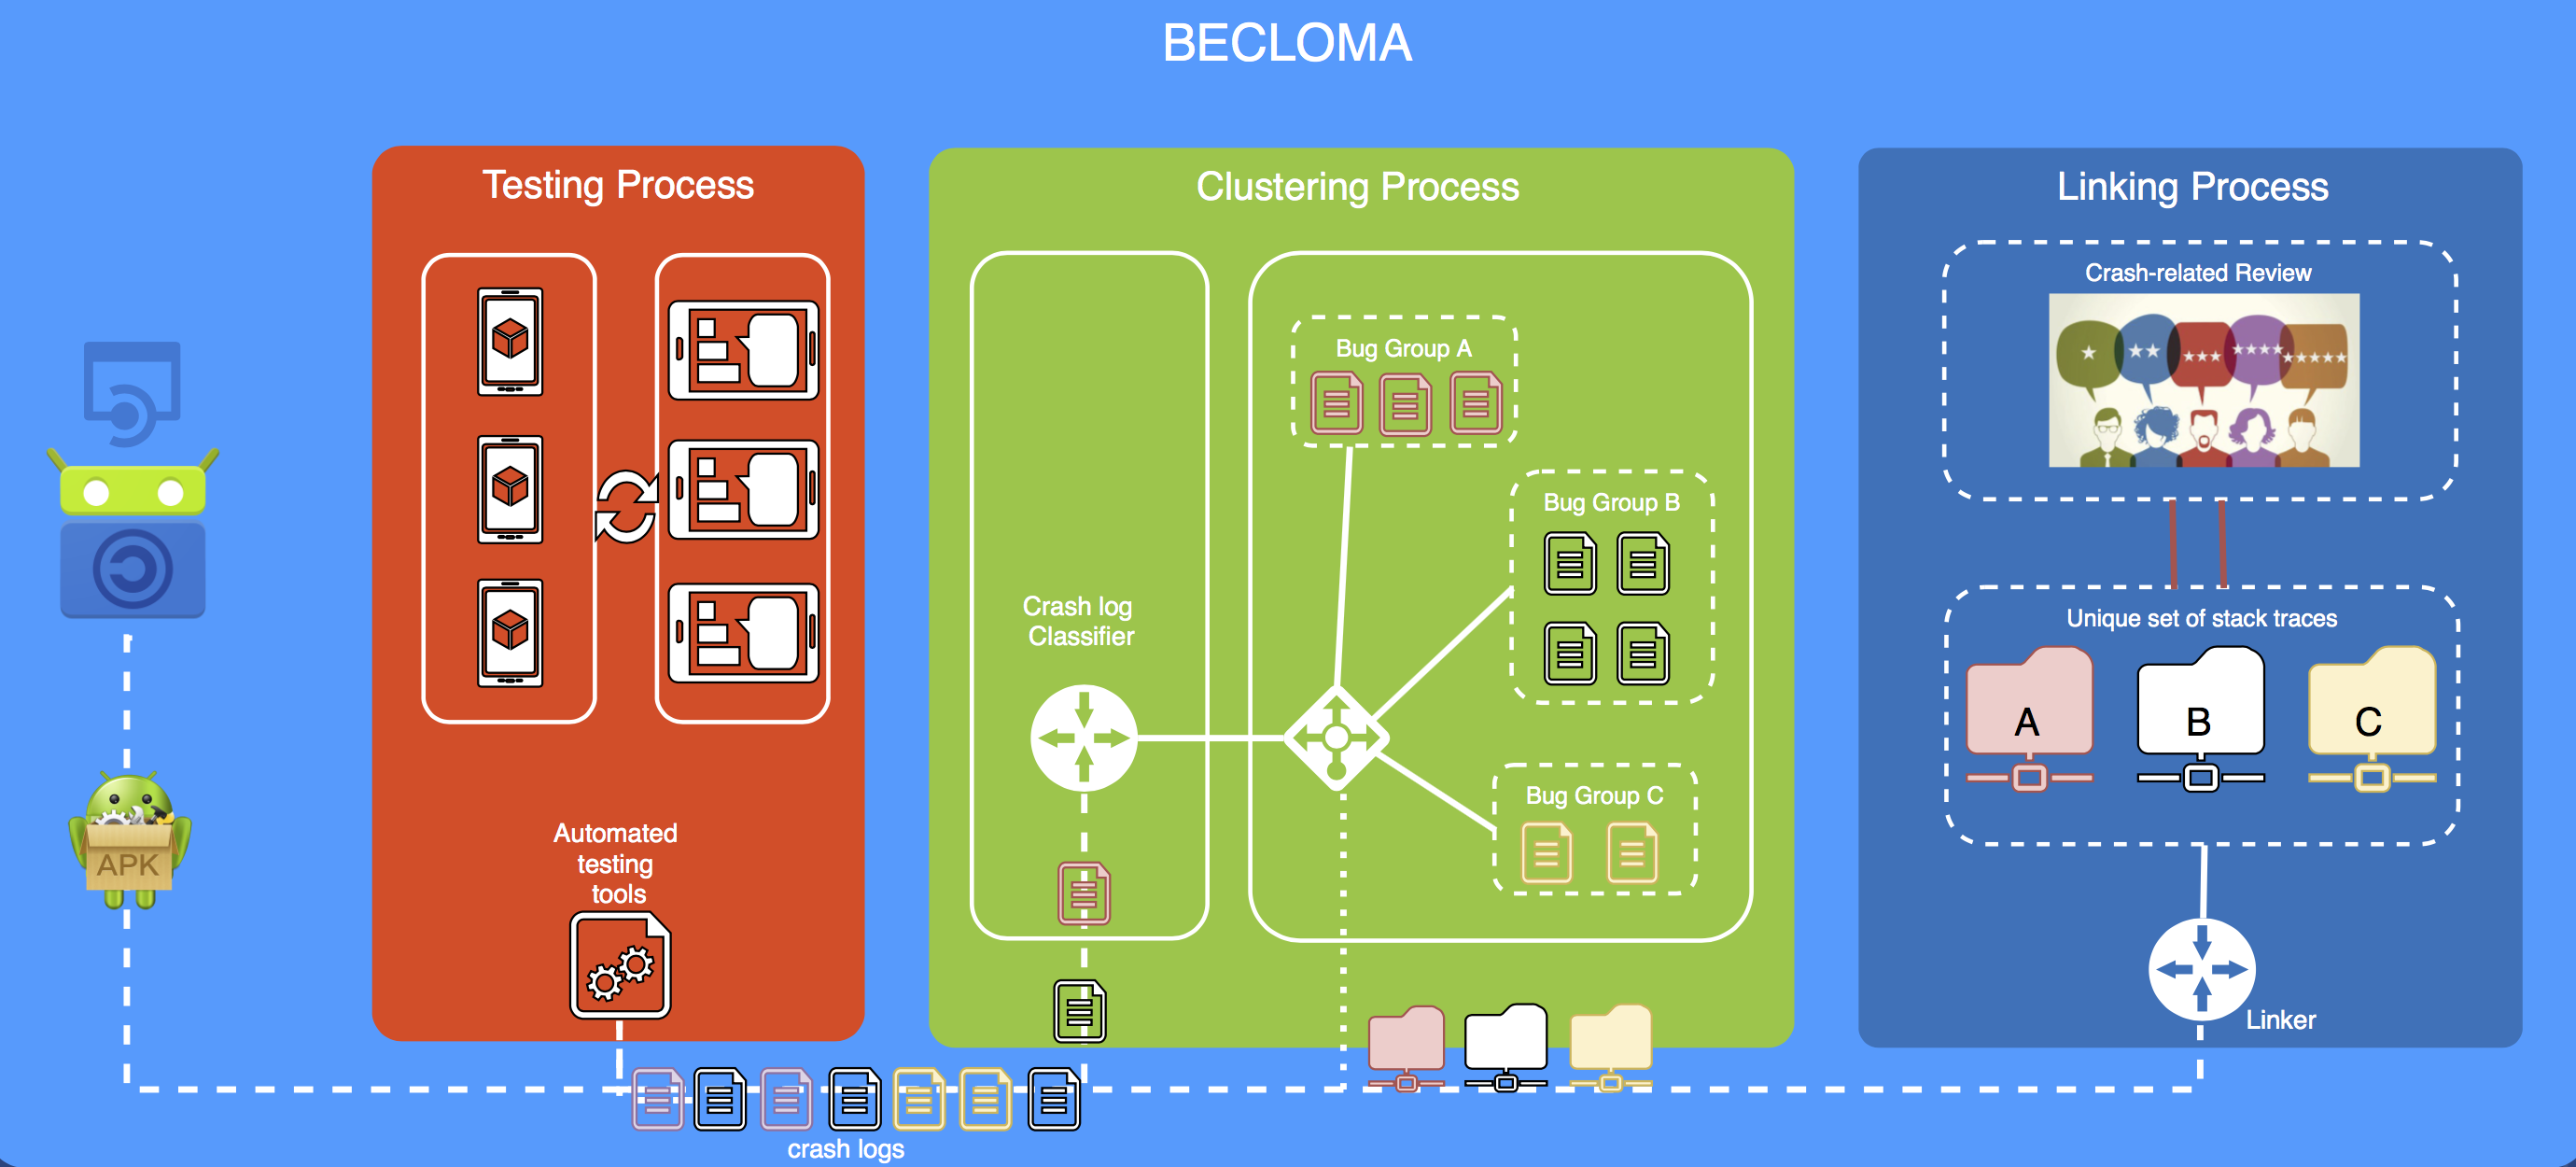
\includegraphics[width=\columnwidth]{diagrams/becloma_approach_img} 
\caption{\toolname\ approach}
\label{fig: becloma}
\end{figure}


\section{Testing and Traces Collection}
\label{approach:testing}
The first step in the overall approach basically relies on two of the most used Android testing tools, in order to exercise the SUT under tests and collect as many failures as possible. 
First of all, \toolname\ acts as crawler in order to download the set of desired \textit{APKs} from the \textit{FDroid} API. 
Thus, it firstly reads a static structured file containing a set of android package names; then, it builds the necessary \textit{HTTP links} in order to download the correspondent \textit{APK} files. 
Once the dataset has been built and some testing parameters have been specified, the testing session can be started. 
The set of parameters that must be specified are described in detail in the Section \ref{usage: settings}.
The overall approach of \toolname\ consists of three testing cycles: 
\begin{enumerate}
\item 
The \textbf{single app} cycle concerning the testing of a single \textit{APK}. It represents the time frame for which each \textit{APK} in the dataset is tested. After that time frame, the approach starts with the testing of the next \textit{APK} indicated in the dataset. 
\item The \textbf{dataset} cycle describing the time spent for testing the \textit{APKs} within the dataset exactly one time for that currently cycle. 
\item The \textbf{session} cycle characterizing a testing session, \ie how many dataset cycles have to be performed. 
\end{enumerate}
The figure \ref{fig: testingapproach} explains the roles of these cycles in the testing approach. 
\begin{figure}[tb]
\centering 
%	\vspace{-1.5mm} 
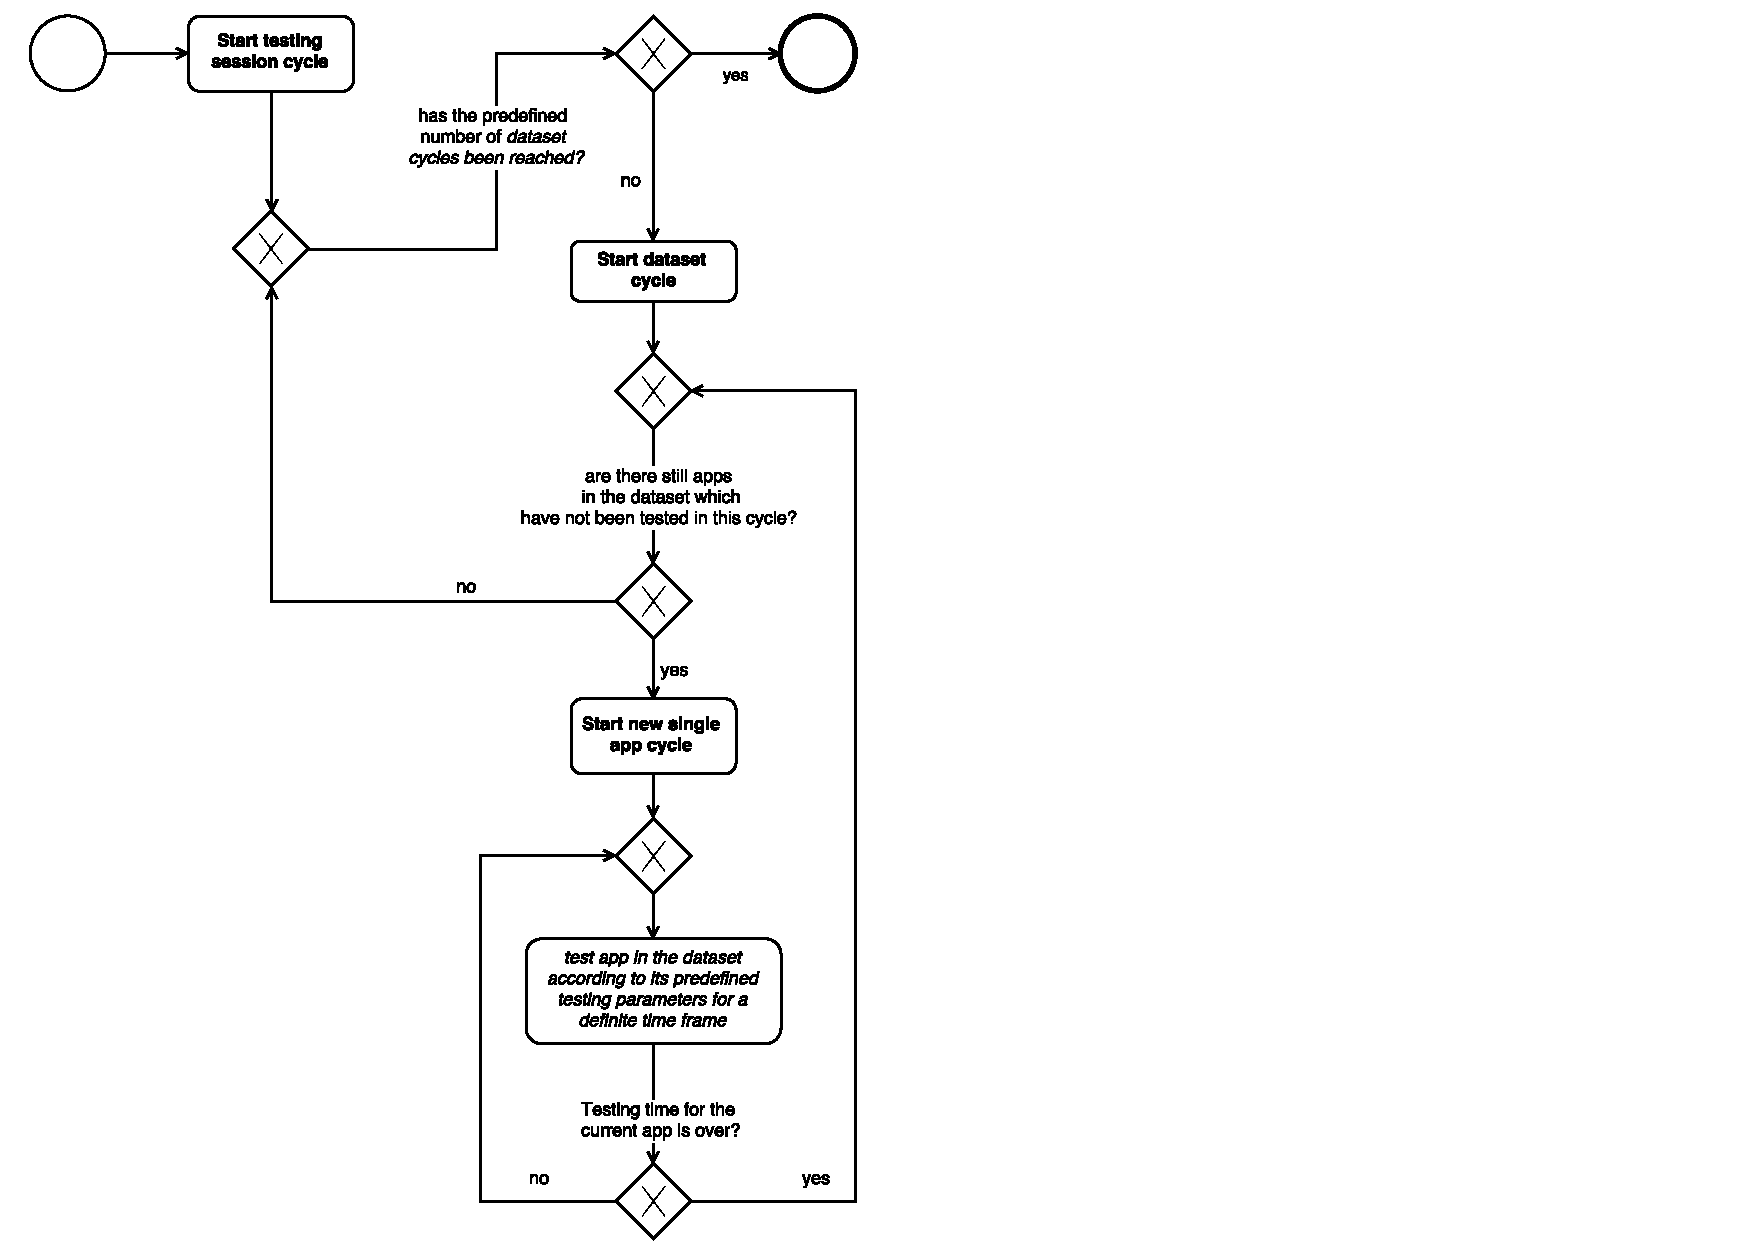
\includegraphics[width=10cm,height=14cm]{diagrams/testingapproach} 
\caption{Testing cycles}
\label{fig: testingapproach}
\end{figure}
The process behind the testing of a single \textit{APK} is illustrated in the figure \ref{fig: apkprocess}.
It tests systemically each \textit{APK} according to its specifications and testing parameters. The former describes the number of random events that will be sent to the app under test, how long the testing of that \textit{APK} will last, the directory where the reports will be stored, etc. 

Once the testing environment has been configured, the test can concretely start. 
After the cycle describing the testing of a single \textit{APK} has finished, \toolname\ begins with the \textit{reporting} phase. 
This step of the approach consists of saving the generated reports which contain the stack traces of the runtime exceptions with the sequence of the events that led to the failures. 
Once the reports of the test has been stored, we proceed to parse them looking for an eventually arose failure. If a crash occurred, we extract its part relative to the stack trace from the whole corpus of the log. At the end, this information is saved into a specific directory aiming at collecting all the arose failures.

\begin{figure}[tb]
\centering 
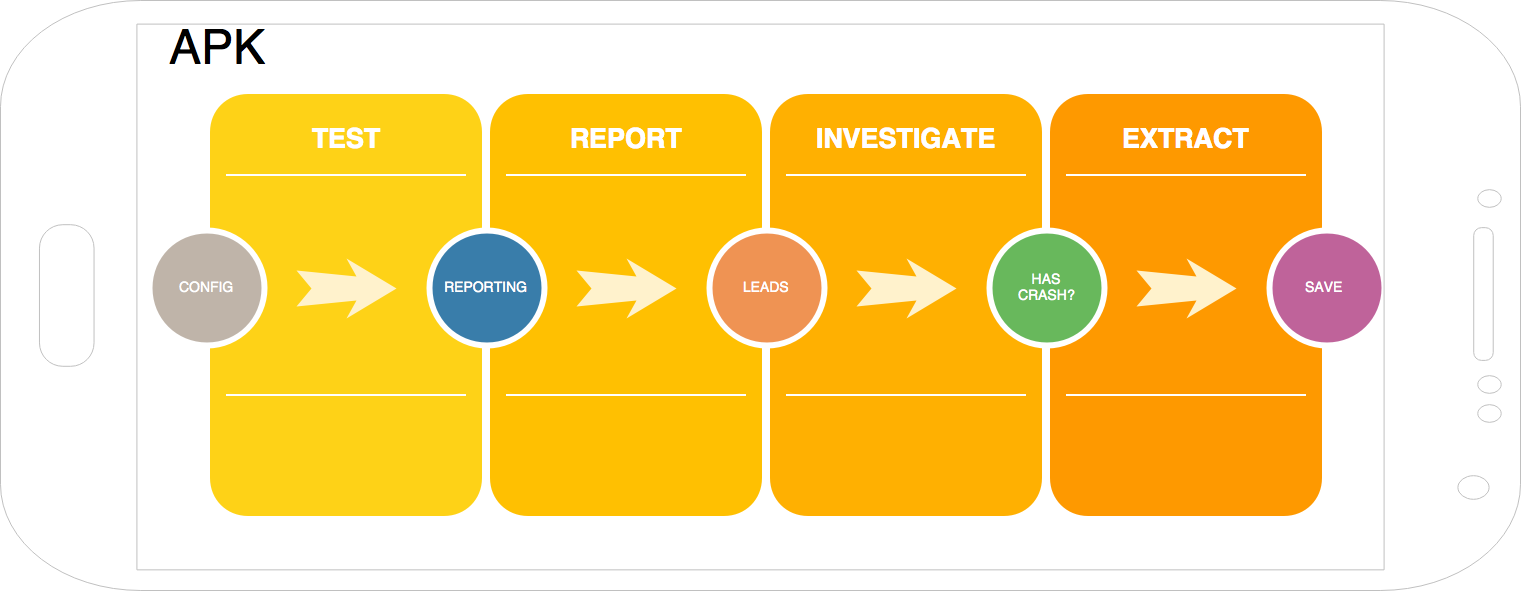
\includegraphics[width=\columnwidth]{imgs/apkprocess} 
\caption{Approach performed by \toolname\ for testing a single android app}
\label{fig: apkprocess}
\end{figure}



%that contain the stack traces of the runtime exceptions detected by the tools together with the sequence of the UI and/or system events that led to the failures [6].



\section{Clustering of The Collected Traces}
\label{approach:clustering}
As we said before at the end of the testing phase all the stack traces that have been generated are stored in a specific directory. However, it is worth to notice that with a high change, most part of such failures would refer to the same bug (in other words, the traces are duplicates).

In order to identify the \textit{unique crashes}, the second step of our approach performs an automatic clustering of the overall bunch of logs. Ideally, at the end of such phase, each cluster should contain logs that refer to the same bug.
For this task, we rely on classic Information Retrieval (IR) techniques, collecting features about the logs and comparing them using the \textit{cosine similarity} metrics (see Section \ref{sec:cosine_similarity}).
Figure \ref{fig: clustering} shows the overall process for this task. 
\begin{figure}[tb]
\centering 
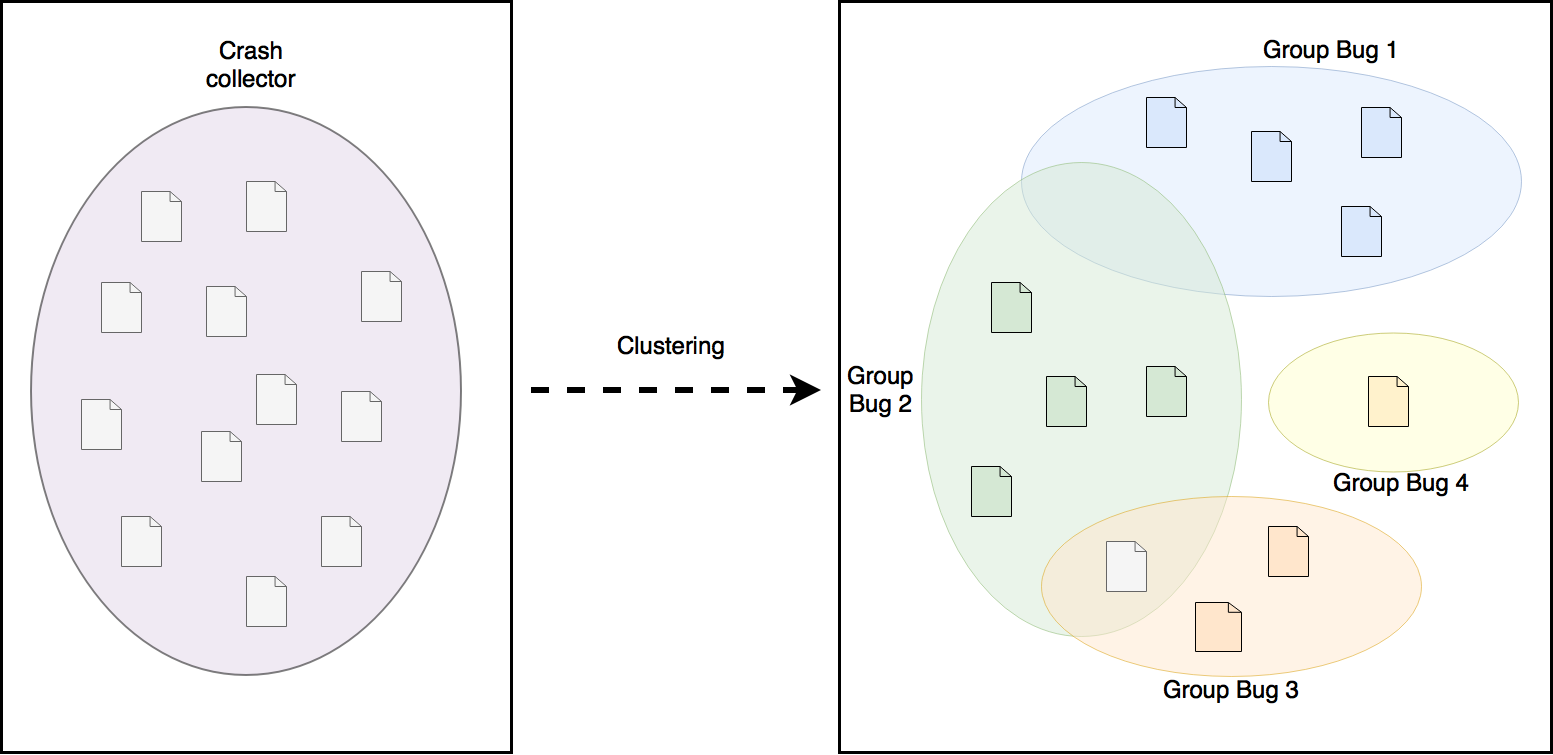
\includegraphics[width=\columnwidth]{imgs/clusteringidea} 
\caption{The idea behind the Clustering process}
\label{fig: clustering}
\end{figure}
As said before, some track traces may be overlapping \ie refer to the same bug of be even duplicates. 
Despite the trigger method, \ie the method that raised to the exception, may be the same, there may be different sequences of function calls in the stack trace, the more the analysis goes deep. 
However, they are hardly detectable and is difficult to affirm that two stack traces which have the same trigger method refer to different bugs. 
Therefore, some reports may belong to two different bug groups in the bucket. 

In order to understand better the Clustering approach, a clarification of how a crash log is structured must be done. 
For this purpose, the real structure of a crash report is illustrated in the listing~\ref{lst: ringdroid}. 
\begin{lstlisting}[caption=Structure of a crash log, basicstyle=\fontsize{6}{8}\ttfamily,label={lst: ringdroid}]
// CRASH: com.ringdroid (pid 6207)
// Short Msg: android.database.StaleDataException
// Long Msg: android.database.StaleDataException: Attempted to access a cursor after it has been closed.
// android.database.StaleDataException: Attempted to access a cursor after it has been closed.
// 	at android.database.BulkCursorToCursorAdaptor.throwIfCursorIsClosed(BulkCursorToCursorAdaptor.java:64)
// 	at android.database.BulkCursorToCursorAdaptor.getCount(BulkCursorToCursorAdaptor.java:70)
...
\end{lstlisting}
A crash log is usually structured as follows: 
\begin{itemize}
\item \textit{Line 1} represents the top of the crash log, where the concerned package name is made explicit;
\item \textit{Line 2} tells in few words the cause of the exception; 
\item \textit{Line 3} complements the cause of the exception giving a long explanation about the exception itself;
\item \textit{Line 4} represents the first line of the stack trace and contains the name and the generic cause of the exception. 
From this point, all the function calls underlying are part of the stack trace;
\item \textit{Line 5} is considered the exact reason for the exception, \ie the trigger method within the source code that caused the crash;
\item From \textit{line 6} moving gradually down until the end of the stack trace, there are other nested function calls which contain additional information about the cause of the exception. Usually, the most important ones for identifying the cause are in the first few lines. 
\end{itemize}
%\GIO{Specify that we used a search based approach to identify the correct threshold to choose whether two logs are the same or not}
In order to state whether two crash reports refer to the same bug or not, we used a search based approach to identify the correct threshold. 
Indeed, we built an \textit{Oracle} which is in charge of comparing two crash logs and is able to answer the following question: \textit{Do they refer to the same bug?}. 
For its answers it makes use of a similarity tolerance, which has been adapted on the base of our experimental results. 
Indeed, we manually created the bucket of unique crash logs and consequently adapted the threshold in the oracle in order to enable it to rightly answer its questions and so reproduce the same bucket. 

\paragraph{Preprocessing.}
The first step of the clustering approach consists of \textit{preprocessing} the crash reports in order to prepare them to be compared to each other. 
To achieve this, the approach follows a grammar-based tokenization technique implemented in the well-know \textbf{Apache Lucene} \cite{lucene} library.  
%Indeed, all words contained in the crash reports are preprocessed using \textbf{Apache}. 
In this direction, we collected all words contained in the crash reports and preprocessed them using a Lucene tokenizer, called \textit{StandardTokenizer}. 
%\GIO{Do not use too often ''the approach consists''! You can use 'it' or 'we'}
This tokenizer simply splits the word fields into lexical units using punctuation and whitespaces as split points. In addition, it removes unnecessary symbols (\eg \texttt{"//"}).
\toolname\ converts all strings to lower-case and extends the tokenizer to a further regular expression. 
This because, it is a worldwide convention that developers use CamelCase notation for writing programming words such as names of classes, names of functions or names of variables.
Since most of the words included in the crash logs are programming language keywords, \toolname\ complements such the StandardTokenizer, so that CamelCase text fields can be also split at the upper-case letters into separate words. 

\paragraph{TF-IDF.} 
Once all words inside the crash logs have been tokenized, we relied on some well know Information Retrieval techniques in order to link together the duplicated crashes.
As features for such process, we relied on the computation of the the \textit{tf-idf} \textit{(term frequency inverse document frequency)} values on the collected stack traces. 
In this direction, \toolname\ computes tf-idf numerical statistics in order to find the relevance of a word in a collection of documents (in our case, the crash logs). Tf-idf is a well-know term-weighting scheme and usually is used in information retrieval or text mining \cite{tfidf}. %Indeed, tf-idf is a way to measure the relevance, the weight of a term compared to its document or its entire document collection (in our case, the crash logs). 
The importance of a term is given by the number of times it occurs in a particular document, inversely proportional to its appearance in the entire documents collection \cite{campbell}. 
%\GIO{The tfidf is not an algorithm. That's a statistics that measure the importance of a word in a set on document. Slightly modify this section changing a bit the terminology}
Generally, a tf-idf scheme consists of three main components \cite{tfidfsimilarity}: 
\begin{itemize}
\item \textbf{TF (Term Frequency)}, \ie how many times a term appears in the currently scored document, where repeated terms indicate the topic of the document; A high TF means that the word in question has a high relevance for the document. The following simplified equation \cite{tfidf} describes a formula for calculating the term frequency:
\begin{align*}
tf_{x,y} = \frac{n_{x,y}}{\mid d_{y} \mid}
\end{align*}
where $n_{x,y}$ represents the number of occurrences of the term $t_x$ in the document $d_{y}$, while $\mid d_{y} \mid$ represents the number of words inside the document $d_{y}$.

\item \textbf{IDF (Inverse Document Frequency)}, \ie the inverse of the document frequency, that represents the number of document in which the term appears. If the same term appears in fewer documents, IDF shows a high value, if a term is very common it returns a low value. 
The equation \cite{tfidf} below describes a simplified version of the inverse document frequency formula: 
\begin{align*}
idf_{x} = \frac{\mid D \mid}{\mid \{d: t_{i} \in d\} \mid}
\end{align*}
where $\mid D \mid$ is the number of documents in the collection, while $\mid \{d: t_{i} \in d\} \mid$ represents the number of documents which contains the term $t_i$

\item \textbf{TF-IDF}, \ie the product of the two above terms. If it has a high value means that the currently scored term has a high relevance, otherwise if it returns a low value, the term has little relevance.
\begin{align*}
tfidf_{x,y} = tf_{x,y}*idf_{x}
\end{align*}

\end{itemize}
The IDF metric actually measures how important a term is. This because, a term which appears very often in a single document will have a high TF score but if this term rarely occurs in the other ones it will also have have a high IDF score and so a low TF-IDF value. This would imply that it shall not have a high relevance. Otherwise, if a word occurs very often both in a single document and in the entire collection it has a high TF score and a low IDF-value, which results in a high TF-IDF score.

At the end of this phase, \toolname\ has created for each crash log its correspondent vector space model, \ie a weighted vector term, where each term indicates a new dimension in the vector and is associated with its correspondent tf-idf value. 


\paragraph{Cosine Similarity.}
\label{sec:cosine_similarity}
To state whether two crash reports refer to the same bug, the approach computes cosine similarity between their previously created vectors space model. 
The cosine similarity is just a measure of similarity between two vectors \cite{cosine} (in our case, two normalized weighted vectors consisting of their tf-idf scores).
Usually, the resulting similarity ranges from -1 to 1, but in the case of information retrieval, since the frequency of the terms are always positive, the returned values range from 0 to 1, where 0 indicates that two documents are completely decorrelated, while 1 means that the words contained inside them are exactly the same.  
The equation describing the cosine similarity between two vectors is as follows: 
\begin{align*}
cosine\:similarity = \cos({\theta}) = \frac{A\cdot{B}}{||A||\:||B||}
\end{align*}
where, in our case $A$ and $B$ are two normalized weighted term vectors consisting of tf-idf values. 
With the term "normalized" is understood that when two weighted vectors are used to compute cosine similarity among them, for each time a word is contained within a vector but not in the other, that term is inserted into the vector that does not contain it by associating a tf-idf score of 0. Furthermore, in doing so the two vectors will have the same length by making the computation of their dot product possible. 



\section{Linking approach}
\label{approach:linking}
\label{par: infusa}
To study the correlation between user reviews and the outcomes of automated testing tools, \toolname\ assumes that the set of user feedback have been already classified in according to a a defined taxonomy and preprocessed.
In order to classify the user feedback according to a given taxonomy (and ad hoch preprocessed) we relied on an approach implemented by Palomba \etal \cite{Palomba2017}. 
Indeed, they proposed some machine learning techniques for automatically classifying a set of user reviews according to a defined taxonomy. 
%\GIO{This is not super correct. In order to classify the user feedback according to a given taxonomy (and ad hoc preprocessed) we relied on the implementation done by Fabio Palomba and Adelina Ciurumelea in the paper that is also in the references. Use such paper as a reference when citing the such approach. The INFUSE-TA tools uses this approach in order to classify the reviews to link them to the logs}.

Furthermore, it performs a systematic Information Retrieval (IR) preprocessing \cite{BaezaYates:1999} on both the user reviews and \textit{augmented} stack traces aimed at (i) correcting mistakes, (ii) expanding contractions (e.g., \textit{can’t} is replaced with \textit{can not}), (iii) filtering nouns and verbs, (iv) removing common words or programming language keywords, and (v) stemming words (e.g., \textit{aiming} is replaced with \textit{aim}). \\
The text below depicts an example of Information Retrieval preprocessing applied on a user feedback: 
\smallbreak
\emph{\small``Crashes on Messages I would give this 5 stars but it crashes every time I try to access my messages in the app. I have removed and reinstalled the app  signed in and out  even reformatted my phone. But it still crashes when I click Messages  every time without fail.''}. 
\smallbreak
Following, the review is preprocessed applying the techniques described above.  
\smallbreak
\emph{\small``crash messag i would give 5 star crash everi time i tri access messag app i remov reinstal app  sign  even reformat phone but still crash i click messag  everi time without fail''}. 
\smallbreak

In this direction, another experimental called \textbf{INFUSE-TA} (\textbf{IN}tegrator o\textbf{F} \textbf{US}er \textbf{FE}edback while Testing \textbf{A}pps) developed by a team at the Software Evolution and Architecture Lab, used the approach proposed by Palomba \etal in order to classify the reviews to link them to the crash reports. 

\paragraph{Linking between Crash Logs and Reviews}
The last step of the approach consists of linking the information from the stack traces contained in the reports to the relevant user reviews. 
However, linking the two sources of information is not at all obvious.
This because, they come from different worlds: user reviews contain natural human language which describe the overall scenario that led to a failure \cite{mernik}, while the stack traces contain technical information about the exceptions raised during the execution of a certain test case. 
To account for this aspect, the approach first removes all information that creates noise in the collected stack traces, only the name and cause of the raised exceptions are selected, \ie the first line of the stack trace (in the example \ref{lst: ringdroid} the \textit{line 4}). 
The choice of considering only some specific parts of the stack traces was driven by experimental results. 
These result illustrated how the linking accuracy was influenced by the presence/absence of this information. 
After cleaning the reports, the remaining text is \textit{augmented} with the source code methods included in the stack trace. 
This concretely means, that each method extracted from the stack trace gets compared with all methods included in the source code. 
If a correlation among them exist, the stack trace is \textit{augmented} with the body and the set of words related to the that method. 
This step extends the information from the reports with contextual information from the source code, possibly providing additional information useful for the linking process. Also in this case, the choice was not random but driven by the experimental results.
Afterwards, the approach performs the systematic Information Retrieval (IR) preprocessing \cite{BaezaYates:1999} \textbf{INFUSA-TA}.
Finally, the resulting documents are linked using the asymmetric Dice similarity coefficient \cite{BaezaYates:1999}, which is defined as
follow: 
\begin{align*}
Dice (review_j, crash_i) = \frac{|W_{review_j} \cap W_{crash_i}|}{\textit{min}(|W_{review_j}|, |W_{crash_i}|)}
\end{align*}
where $W_{review_j}$ represents the set of words composing a user review $j$, $W_{crash_i}$ is the set of words contained in an augmented stack trace $i$ and the $min$ function normalizes the Dice score with respect to the number of words contained in the shortest document between $j$ and $i$. 
The asymmetric Dice similarity returns values between [0,1]. 
In my thesis, pairs of documents having a Dice score higher than \textbf{0.5} were considered as linked by the approach.








\chapter{\toolname}
The tool I implemented, called \toolname, is a \textit{java-based} tool aimed at helping further developers during the testing process of their Android mobile applications. \\
For giving a cleaner and more understandable explanation of how \toolname\ works, I would like to split its key features into three main categories (which should also be executed in a sequential way, in order to exploit the whole \toolname's potentiality): 
\begin{enumerate}
\item the \textsc{Testing} part is in charge of testing a given set of \textit{APKs}, reporting their testing results and extracting possible \textit{crashes} from the before generated test logs; 

\item the \textsc{Clustering} part investigates the similarity between the previous extracted crash logs, using different metrics and strategies, in order to collect they together and create a crash log \textit{bucket}; 

\item the \textsc{Linking} part represents the core feature of \toolname. It pre-processes a set of given \textit{user reviews} as well as the set of the previously created crash logs, in order to prepare and "clean" them for the linking procedure.  Afterwards, it investigates whether it exists a correlation between the stack traces and the user feedbacks, with the aim to link, whether possible, the reviews with the crash logs. 
\end{enumerate}

\section{Testing}
%----------------- FDROID CRAWLER --------------
First of all, if no set of \textit{APKs} is available yet, \toolname\ can be exploited for downloading the needed mobile applications from the \textit{F-Droid API\footnote{LINK API}}. In this direction, as shown in the picture \ref{testing}, the component \FDroidCrawler, is first in charge of  parsing a static structured file (\textit{e.g.} a \textit{csv}-file format), which contains a set of android packages names. 
The path of this file is given in the \textsc{configuration manager}, which contains a set of static properties that get elaborated by \toolname. Second, \textsc{fdroid crawler} searches and then extracts a set of \textit{HTTP links} for those android packages that have been found on the API. Afterwards, it builds the correct \textit{HTTP requests} and finally starts the downloading process, saving the returned \textit{APKs} in a given directory.

%-------------- CONFIGURATION ENVIRONMENT--------------
The first step of the testing part was to build a set of \textit{APKs}, with which to perform the testing process. As said, this can be achieved using either \textsc{fdroid crawler} or can also be manually created. Now, the second step is to prepare and configure the testing environment. 
All the parameters needed for starting a testing session have to be specified in the \textsc{configuration manager}. Figure \ref{config}, shows an example of a simplified set of parameters which must be given a priori in order to launch a testing session. \newpage
\label{config}
\begin{lstlisting}[caption=Properties which get elaborated during the testing sessions]
/**
 * Testing session specifications
 */
MINUTES_PER_APP = 30
NR_OF_ITERATIONS = 5
 
/**
* Test logs directories
*/
MONKEY_DIR = Reports/MonkeyReports
SAPIENZ_DIR = Reports/SapienzReports

/**
 * Monkey parameters
 */
LOG_VERBOSITY = -v 
PACKAGE_ALLOWED = -p
NR_INJECTED_EVENTS = 5000
DELAY_BETWEEN_EVENTS = 10
PERCENTAGE_TOUCH_EVENTS = 15
PERCENTAGE_SYSTEM_EVENTS = 15
PERCENTAGE_MOTION_EVENTS = 15
IGNORE_CRASH = True

/**
* Sapienz parameters
*/
SEQUENCE_LENGTH_MIN = 20
SEQUENCE_LENGTH_MAX = 500
SUITE_SIZE = 5
POPULATION_SIZE = 50
OFFSPRING_SIZE = 50
GENERATION = 100
CXPB = 0.7
MUTPB = 0.3
\end{lstlisting}
The figure above represents a part of the \textsc{configuration manager}, where all the testing parameters for \monkey and \sapienz are specified. An in-depth explanation about these parameters concering \monkey and \sapienz can be found on \cite{monkey}, respectively on \cite{sapienz}.\\
In addition to them, the directories on which the generated test logs are going to be stored must be given as well as the specifications about the testing session. The properties about the testing session consist of two values: 
\begin{itemize}
\item \textsc{minutes\_per\_app}, specifies how many minutes an app will be tested. After that time frame, a time-out occurs and the testing process gets restarted with the next app. 
\item \textsc{nr\_of\_iterations}, specifies how many times the whole dataset will be tested.
\end{itemize}

According to the example \ref{config} above and assuming that the \textit{APKs} set consists in 10 apps, the total estimated testing time for an entire testing session would be: 
\begin{center}
30 min p/a * 10 apps * 5 iterations = 1500 min. (25 hours). 
\end{center}
Once the environment testing variables have been configured, the automated tool with whom the testing is going to be performed must be made explicit. Indeed, it has to be specified as parameter in \textsc{main} \textit{args} (as mentioned before in the section \ref{sec:choicetool}, the tools which can be selected are either \monkey or \sapienz). \\
The last configuration step is to define on which kind of device (\textit{i.e}, a real device, such as a \textit{tablet} or a virtual device, such as an \textit{emulator}) the testing is going to be performed. In addition to them, an additional argument that starts a timer for a better overview during the testing process can also be passed as main argument. \toolname\ supports different types of emulators or real devices running on different android API levels. However, in order to correctly execute \sapienz, the API level shall be the \textit{Android 4.4, KitKat}. \\
The listing below shows an example of a combination of possible parameters that could be given as main arguments. 


\begin{lstlisting}[caption=\toolname\ command line, language=bash]
$ java -\toolname.jar -device -monkey -timer
\end{lstlisting}

%-----------LAUNCH A TESTING SESSION -----------
Once the configuration phase is terminated, \toolname\ is able to start the testing process. 
As shown in the picture \ref{testing}, it manages the component \SessionLauncher, which is in charge of translating the previously specified testing properties into "java readable code" and initializing the testing session. 
Concretely, after \toolname\ invokes \SessionLauncher\ all the attached devices respectively the chosen emulators get initialized, \ie they get rebooted and restarted as root, so that some important write-read-permissions are enabled during the testing session. 
Whether the timer has been given as main argument, it gets also started. \\
Once the initialization step has been completed, \SessionLauncher\  invokes the \AppTester\ component which finally starts the testing session. The Listing~\ref{lst:startsession} gives a simplified code snippet about the beginning of the testing process. 

\begin{lstlisting}[caption=\SessionLauncher\ Code snippet for starting a testing session, ,label={lst:startsession}]
private appTester; 
public void startTestingSession() throws Exception {
        final int NUMBER_ITERATIONS = ConfigurationManager.getNumberOfIterations();
        if (IS_EMULATOR) {
        	   SessionLauncher.initialiseEmulator();
        }
        else {
       	   SessionLauncher.initialiseDevices();
        }
       
        if (isTimer) {
            SessionLauncher.initializeTimer();
        }
        for (int i = 0; i < NUMBER_ITERATIONS; i++) {
            System.out.println("Iteration number " + (i+1));
            this.appTester = new AppTester();
            this.appTester.testAllApp();
        }
}
\end{lstlisting}
First of all, the total number of iterations specified in the \Config\ is read and stored into a constant of type int. After that, all the attached devices (or the chosen emulators) gets statically initialized. According to the boolean variable \textit{isTimer}, a timer may also be started.
Afterwards, a for-loop starts where at each iteration the method \textit{testAllApp()} gets invoked. 
The idea behind this, is that at each iteration a new object of type \AppTester\ is created, so that each created object represents one testing loop of the dataset. 
For this reason, as shown in the figure~\ref{testing}, the \SessionLauncher\ would be able to instantiate infinite times the class \AppTester. However, it must create at least one object of that type in order to start a testing session. 

\AppTester\ and \Cmd\ represent the core components of the whole testing process. Indeed, \AppTester\ can be viewed as brain of the process, since it tells step-by-step to the body, \ie the \Cmd\ component, which commands it has to execute and at what stage of the process it has to perform it. \\
Listing~\ref{lst:apptester} shows a very simplified code snippet of the relation between the two above mentioned components. 
\begin{lstlisting}[caption=Testing mechanism between \AppTester\ and \Cmd\, ,label={lst:apptester}]
/**
* @class: AppTester
*/
public void testAllApp() {
        for (File apk : this.apksDirectory) {
            if (apk.getName().endsWith(".apk") && !apk.isDirectory()) {
                    uninstallApp(apk.getName());
                    installApp(apk.getName());
                    if (IS_MONKEY) {
                        testAppWithMonkey(config.getMonkeyRepDir(), apk.getName());
                    } else if (IS_SAPIENZ) {
                        testAppWithSapienz(config.getSapienzRepDir(), apk.getName());
                    }
            }
        } 
        // waiting to threads to finish 
        File testLog = CmdExecutor.getCurrentLog();
        if (hasCrash(testLog)) {
            generateCrashLog(testLog);
        }
} 
private void testAppWithSapienz(String dest, final String APK_NAME) {
	CmdExecutor.generateReport(dest, CommandLines.SAPIENZ_CMD_LINE(APK_NAME)); 
}

private void testAppWithMonkey(String dest, final String APK_NAME) {
	CmdExecutor.generateReport(dest, CommandLines.MONKEY_CMD_LINE(APK_NAME)); 
}

/**
* @class: CmdExectutor
*/
public static void generateReport(String dest, String cmd){
        Runtime runtime = Runtime.getRuntime();
        Process p = runtime.exec(cmd);
        StreamGobbler output = new StreamGobbler(p.getInputStream(), cmd, dest); 
        output.start();
        writeTestingEndTime(dest);
    }
    
public static File getCurrentLog() {
    return lastGeneratedLog();
}
    
\end{lstlisting}


First of all, \AppTester\ creates a for-loop in which it iterates each \textit{APK} file contained in the \textit{APKs} directory. Once again, this directory is specified in the \Config. 
The first if statement checks whether the file in question has an adequate extension, \ie it is able to be installed on a android mobile device. After that, \AppTester\ uninstalls the concerned \textit{APK}, so that at each iteration of the testing it get reinstalled. This beacause, it may be that an \textit{APK} gets affected by previously generated sequences (\eg a sequence of random events that led the app to an external website). \\
Afterwards, \AppTester\ checks which automated tool has been chosen by the tester, so that it can tell to the \Cmd\ component, which command-line it has to execute. As stated before, \AppTester\ prepares the single testing components such as which \textit{APK}, which tool, which testing parameters, etc., while \Cmd\ executes them without any prior knowledge. \\
After the automated tool has been detected, \Cmd\ is able to concretely start the testing, executing the passed command-line. This is represented in listing \ref{lst:apptester} by the method \textit{generateReport}. Indeed, \Cmd\ uses a single instance of the java-class \textit{Runtime} that allows the application to interact with the environment in which the app is running \cite{runtime}. This is actually achieved by the \textit{Runtime.getRuntime()}. The next line executes with the previously created object the given command-line. Since this method returns a new Process object, the result of the execution is assigned to a separate process. \\
Assigning the execution of each single command-line to a new single separate process brings with it many advantages: 
\begin{itemize}
\item Processes are independent of each other. If the execution of a command-line fails, it can be interrupted without affecting the entire testing process; 
\item Multithreading can be easily supported; Indeed, the component \Stream\ extends the \textit{Thread} java-class which implements the \textit{Runnable} java-interface. Each time a new process comes in, it starts a new thread in this class.
\item Each process has it own timeout. It may be that some command-lines cannot properly terminate and need to be interrupted during their execution.  
\end{itemize}
\Stream, in turn, is in charge of writing the test report. Each time its construct get instantiated in the \textit{generateReport()} method of the \Cmd\ class, it starts a new thread and begins in parallel the writing phase of the log. 
As shown in listing~\ref{lst:gobbler}, the method \textit{run()} overridden from the \textit{Runnable} interface gets automatically per-default invoked when in the \textit{generateReport} method an object of type \textit{StreamGobbler} calls the \textit{start()} method. 
Once the \textit{start()} method is called, the writing phase starts. This phase uses a \textit{PrintWriter} as well as classic \textit{Reader} for writing text on a file.
Before the test log is written, the metadata about the testing environments are appended to the writer. At the end of the process the writer is closed and the thread can terminate. Once the thread is finished, the method \textit{writeTestingEndTime()} in the method \textit{generateReport()} can start. This method complement the metadata writing the testing end time, so that the total testing time can be computed. 





\begin{lstlisting}[caption=\Stream\ code snippet writing a test log, ,label={lst:gobbler}]
/**
* @class: StreamGobbler
*/
@Override
public void run() {
        try {
            Writer writer = new PrintWriter(outputPath, "UTF-8");
            InputStreamReader isr = new InputStreamReader(is);
            BufferedReader br = new BufferedReader(isr);
            String line;
            writer.append(TesterData.getMetaData()); // insert metadata
            while ((line = br.readLine()) != null) {
                System.out.println(" > " + line); // console overview
                writer.append(line).append("\n"); // test log 
            }
            closeWriter();
        } catch (IOException ioe) {
            ioe.printStackTrace();
        }
}
\end{lstlisting}

Listing~\ref{lst:testinglog} shows a short version of a test log of the app \textit{com.danvelazsco.fbwrapper} that has been generated after the execution of \monkey. 

\begin{lstlisting}[caption=Test log of com.danvelazco.fbwrapper, basicstyle=\fontsize{7}{8}\ttfamily,label={lst:testinglog}]
/**
 * Meta-data
 */
Tester Name: Lucas Pelloni
Testing Start Time: 05/04/2017 11:18:29
Testing End Time: 05/04/2017 11:48:30
Total Testing Time: 30 minutes (0.5 hours)
Type of testing: testing on a physical device
Device name: c0808bf731ab321
Percentage of motion events: 2.0% (number of motion events: 60 of 3000 events)
Percentage of system events: 6.0% (number of system events: 180 of 3000 events)
Percentage of touch events: 1.0% (number of touch events: 30 of 3000 events)

/**
 * Test log 
 **/
:Monkey: seed=1495075565065 count=3000
:AllowPackage: com.danvelazco.fbwrapper
:IncludeCategory: android.intent.category.LAUNCHER
:IncludeCategory: android.intent.category.MONKEY
// Event percentages:
//   0: 1.0%
//   1: 2.0%
//   2: 2.4931507%
//   3: 18.698631%
//   4: -0.0%
//   5: 31.164383%
//   6: 18.698631%
//   7: 6.0%
//   8: 2.4931507%
//   9: 1.2465754%
//   10: 16.205479%
:Switch: #Intent;action=android.intent.action.MAIN;category=android.intent.category.LAUNCHER;end
    // Allowing start of Intent { act=android.intent.action.MAIN cat=[android.intent.category.LAUNCHER]
:Sending Trackball (ACTION_MOVE): 0:(4.0,4.0)
:Sending Trackball (ACTION_MOVE): 0:(4.0,-3.0)
:Sending Trackball (ACTION_MOVE): 0:(2.0,-1.0)
:Sending Trackball (ACTION_MOVE): 0:(-5.0,2.0)
:Sending Trackball (ACTION_MOVE): 0:(-5.0,3.0)
    //[calendar_time:2017-05-05 09:48:23.894  system_uptime:717348]
    // Sending event #100
...
\end{lstlisting}

As shown in the figure above, the test logs do not only contain the test results of the tested app, but also the above mentioned meta-data for documenting and retracing the whole testing session.

The testing phase in the "strict sense", \ie the stage where the \textit{APK} gets stressed with an automated tool is over. At this point, the logs must be investigated about the possibility that some apps have generated a crash during its testing time frame. In this sense, the last part of the method \textit{testAllApp()} illustrated in the listing ~\ref{lst:apptester}, is in charge of stating whether a test log contains a crash or not. The method for checking whether a test log has collected a crash inside it is quite intuitive. This because, the syntax used by \monkey and \sapienz in their report for indicating the presence of a crash is the same. As illustrated in the listing~\ref{lst:crashlog}, a crash can be delimited using the following two \textit{Strings}: 
\begin{itemize}
\item Crash beginning: \texttt{"// CRASH: "}
\item Crash end: \texttt{"// "}
\end{itemize}

\begin{lstlisting}[caption=Crash log of com.danvelazco.fbwrapper illustrated within its test log, basicstyle=\fontsize{6}{8}\ttfamily,label={lst:crashlog}]
...
:Sending Trackball (ACTION_MOVE): 0:(3.0,3.0)
:Sending Trackball (ACTION_MOVE): 0:(-4.0,-3.0)
:Sending Trackball (ACTION_MOVE): 0:(3.0,-1.0)
// CRASH: com.danvelazco.fbwrapper (pid 4302)
// Short Msg: java.lang.NullPointerException
// Long Msg: java.lang.NullPointerException
// Build Label: samsung/espressowifixx/espressowifi:4.2.2/JDQ39/P3110XXDMH1:user/release-keys
// Build Changelist: 8291
// Build Time: 1419156873000
// java.lang.NullPointerException
// 	at com.danvelazco.fbwrapper.activity.BaseFacebookWebViewActivity.onKeyDown(BaseFacebookWebViewActivity.java:649)
// 	at com.danvelazco.fbwrapper.FbWrapper.onKeyDown(FbWrapper.java:429)
// 	at android.view.KeyEvent.dispatch(KeyEvent.java:2640)
// 	at android.app.Activity.dispatchKeyEvent(Activity.java:2433)
// 	at com.android.internal.policy.impl.PhoneWindow$DecorView.dispatchKeyEvent(PhoneWindow.java:2021)
// 	at android.view.ViewRootImpl$ViewPostImeInputStage.processKeyEvent(ViewRootImpl.java:3845)
// 	at android.view.ViewRootImpl$ViewPostImeInputStage.onProcess(ViewRootImpl.java:3819)
// 	at android.view.ViewRootImpl$InputStage.deliver(ViewRootImpl.java:3392)
// 	at android.view.ViewRootImpl$InputStage.onDeliverToNext(ViewRootImpl.java:3442)
//     ...
//
:Sending Touch (ACTION_DOWN): 0:(215.0,683.0)
:Sending Touch (ACTION_UP): 0:(163.15541,597.4464)
:Sending Touch (ACTION_DOWN): 0:(243.0,812.0)
...

\end{lstlisting} 
Indeed, the method \textit{generateCrashLog()} (~\ref{lst:generatecrash} in the \textit{testAllApp()} is in charge of extracting the crash(es) from its test log. The parsing technique used by this method is to individuate the beginning of the crash using the \texttt{"START\_CRASH"}  string. Once the start has been individuated, the loop continues to add lines of the log	until it finds the \texttt{"END\_CRASH"} string. Once the end has been reached the loop terminates and \Cmd\ writes the results into an external file, in order to extract the crash. 

\begin{lstlisting}[caption=\AppTester's method for extracting a crash log from its test log,label={lst:generatecrash}]
/**
* @class: AppTester
*/
public void generateCrashLog(File testLog) {
        ...
        ArrayList<String> crashLog = new ArrayList<>();
        Pattern start = Pattern.compile(START_CRASH);
        String line;
        while ((line = in.readLine()) != null) {
            Matcher matcher = start.matcher(line);
            if (matcher.find()) {  // crash start
                while (!line.contains(END_CRASH)) { // crash end
                    crashLog.add(line);
                    line = in.readLine();
                }
            }
        }
        CmdExecutor.writeToFile(crashLog, dest);
    }
\end{lstlisting} 


At this point, the \textit{APK} has been tested, reported, its test logs have been investigated and possible crashes have been extracted. Figure~\ref{fig: apkprocess} summarizes the four components which characterizes the testing process of one application. 
\begin{figure}[htb]
\centering 
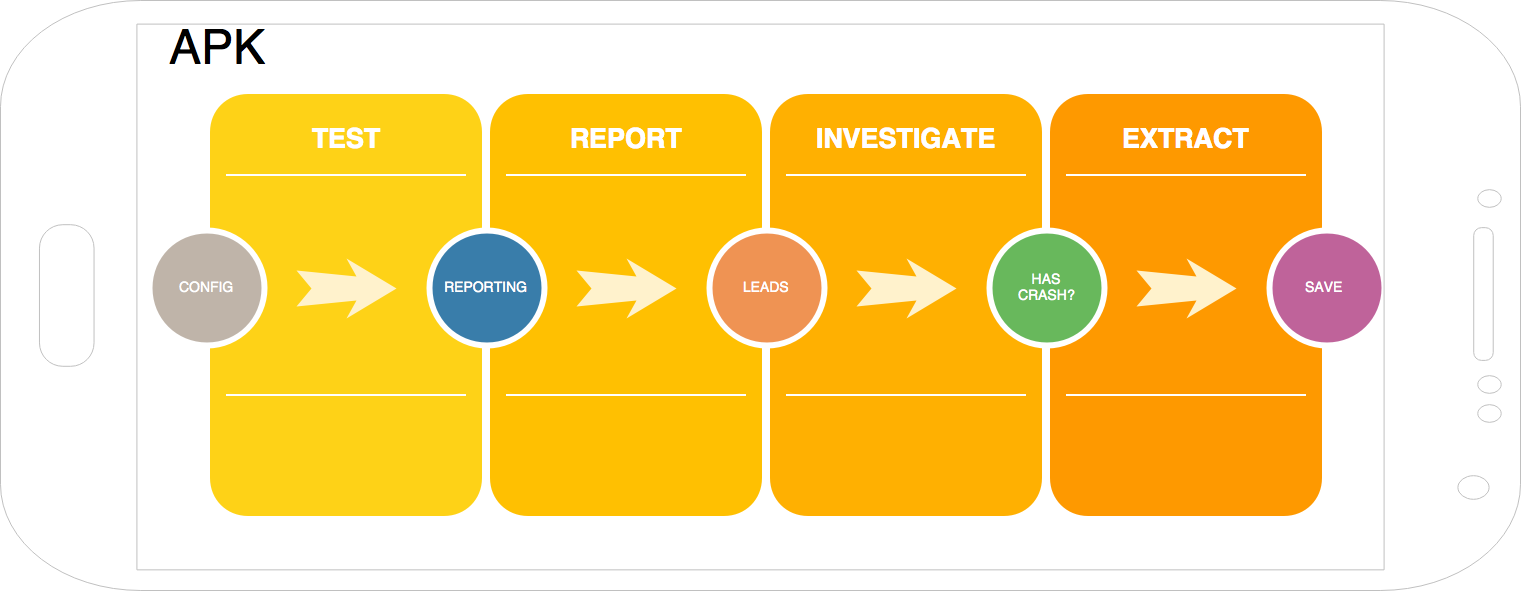
\includegraphics[width=\columnwidth]{imgs/apkprocess} 
\caption{Four test steps performed by \toolname\ of an application}
\label{fig: apkprocess}
\end{figure}



Now, \toolname\ is able to start testing the next application (\ie the next iteration of the loop inside the method \textit{testAllApp())}. 
Once all the applications specified in the dataset have been tested exactly one time, \SessionLauncher\ can begin with the next iteration of its loop (listing ~\ref{lst:startsession}) and so start testing the whole dataset another time. 
This loop ends when the number of iterations reaches the one specified by the user. \\
In addition, during each test iteration and at the end of the whole testing session useful statistics are computed and written into external excel files, using the components \textsc{OnGoingCalculator} and \textsc{FinalCalculator}. They use the pure Java library \textit{Apache POI}, for reading and writing files in Microsoft Office formats \cite{apachepoi}. 




\section{Clustering}
%--------------CLUSTERING AIM-------------
Once the testing phase is finished, all the generated crash logs are stored in a given directory. After this phase, the only way to differentiate them inside this directory is the name of the package for which these crashes occurred. However, among these crash logs there may be a lot of redundancy, since more of them may refer to the same bug. The aim behind the Clustering phase is to create a bucket of unique crash logs. This means, that each crash log has to be compared with the others	 of the same package and according to some metrics that will be explained below, they must be smartly group together. Figure~\ref{fig: clustering} shows the idea behind the Clustering process. 
\begin{figure}[htb]
\centering 
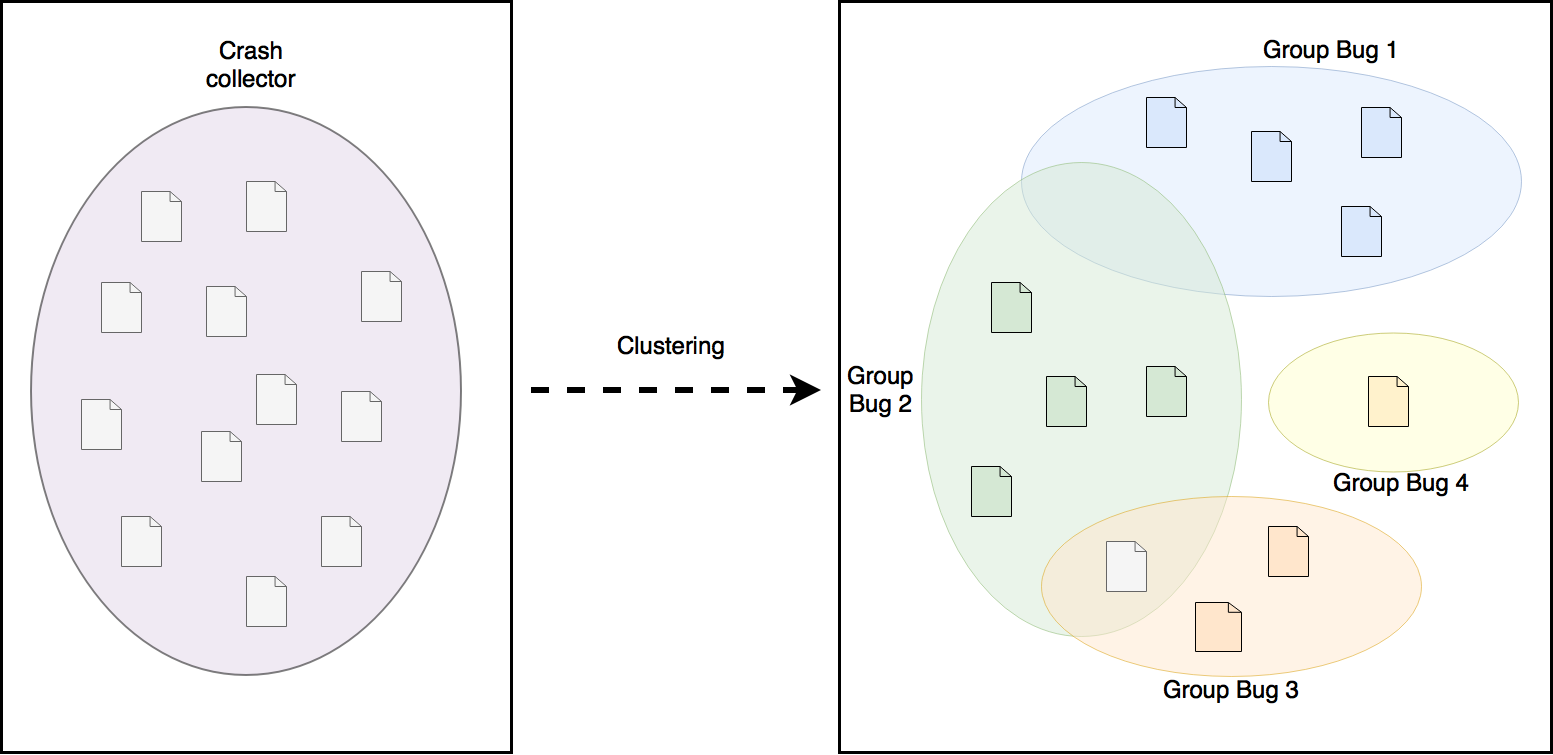
\includegraphics[width=\columnwidth]{imgs/clusteringidea} 
\caption{The idea behind the Clustering process}
\label{fig: clustering}
\end{figure}

Some groups of crash logs may be overlapping. Despite the trigger method, \ie the method that raised to the exception, may be the same, there may be different sequences of function calls in the stack trace, the more the analysis goes deep. However, they are hardly detectable and is difficult to affirm that two stack traces which have the same trigger method refer to different bugs. 

In order to understand better the Clustering approach, a clarification of how a crash log is structured must be done. In order to do this, another example of a crash log is given in the listing~\ref{lst: ringdroid}. 
\begin{lstlisting}[caption=Structure of a crash log, basicstyle=\fontsize{6}{8}\ttfamily,label={lst: ringdroid}]
1.		// CRASH: com.ringdroid (pid 6207)
2.		// Short Msg: android.database.StaleDataException
3.		// Long Msg: android.database.StaleDataException: Attempted to access a cursor after it has been closed.
4.		// android.database.StaleDataException: Attempted to access a cursor after it has been closed.
5.		// 	at android.database.BulkCursorToCursorAdaptor.throwIfCursorIsClosed(BulkCursorToCursorAdaptor.java:64)
6. 		// 	at android.database.BulkCursorToCursorAdaptor.getCount(BulkCursorToCursorAdaptor.java:70)
7.		...
\end{lstlisting}
A crash log is usually structured as follows: 
\begin{itemize}
\item \textit{Line 1} represents the top of the crash log, where the concerned package name is made explicit;
\item \textit{Line 2} tells in few words the cause of the exception; 
\item \textit{Line 3} complements the cause of the exception giving a long explanation about the exception itself;
\item \textit{Line 4} represents the first line of the stack trace. From this point, all the function calls underlying are part of the stack trace;
\item \textit{Line 5} is considered the exact reason for the exception, \ie the trigger method that caused the crash;
\item From \textit{line 6} moving gradually down until the end of the stack trace, there are other nested function calls which contain additional information about the cause of the exception. Usually, the most important ones for identifying the cause are in the first few lines. 
\end{itemize}
Before the explanation of the Clustering process, a premise must be made. All the classes that will be discussed below, refer to the class diagram represented in the figure~\ref{clustering}. 
%TODO aggiungere construttore in crash log passandogli gli argomenti
First of all, \toolname\ individuates the directory in which all the previously generated crash logs have been stored. This directory is indicated again in the \Config.\\  
As shown in the listing~\ref{lst: extractor}, \toolname\ loops all the crashes contained inside it and for each of them it calls the method \textit{extractCrashLog()}, in the \Extractor\ component. 

\begin{lstlisting}[caption=\Extractor\ code snippet converting crash files into CrashLog objects,label={lst: extractor}]
/**
* @class: Main
*/
CrashLogExtractor extractor = new CrashLogExtractor();
final String CRASH_CONTAINER = ConfigurationManager.getCrashContainerDirectory();
File[] crash_container = new File(CRASH_CONTAINER).listFiles();
for (File crash : crash_container) {
	extractor.extractCrashLog(crash);
}
\end{lstlisting} 
The method \textit{extractCrashLog()} converts simple crash log files stored inside a folder into \Crash\ Java-objects. 
Indeed, for each crash log file found inside the directory, the constructor of the \Crash\ class get instantiated and so a new object of this type gets created. Each time the constructor of the \Crash\ class gets invoked, it automatically creates the structure of the \textit{CrashLog objects} analogously to the structure of the real crash log file. \\
For instance, the crash log described in the listing \ref{lst: ringdroid} is converted into the following \Crash-object: 

\begin{lstlisting}[caption=\Crash-object,basicstyle=\fontsize{6}{8}\ttfamily, label={lst: crashobject}]
Crash {
	crash_path = /Users/Lucas/Desktop/UZH/BA/CrashLogCollector/crash_log_com.ringdroid.txt
	packageName = com.ringdroid
	Short = android.database.StaleDataException
	Long = android.database.StaleDataException: Attempted to access a cursor after it has been closed.
	first_java_trace_line = android.database.StaleDataException: Attempted to access a cursor after it has been closed.
	trigger_method = [android.database.BulkCursorToCursorAdaptor.getCount(BulkCursorToCursorAdaptor.java:70)]
	trigger_class = BulkCursorToCursorAdaptor
	all_stack_trace_methods = [BulkCursorToCursorAdaptor, CursorWrapper, MergeCursor,
	 						  CursorAdapter, AdapterView, AbsListView, ViewGroup, Handler, Looper, ActivityThread, 
	 						  Method, ZygoteInit]
	augmented_stack_traces = android database stale attempted access cursor 
						     closed bulk adaptor count wrapper merge widget adapter 
}
\end{lstlisting}



%tf–idf is a way to normalize a token based on both on its occurrence in a particular document (in our case, crash reports), and inversely proportional to its appearance in all documents \cite{campbell}. 



\section{Linking}


\section{How to start \toolname}
First of all, a set of parameters and directories have to inserted in the static \textit{Configuration Manager} file.
% qui inserire la command-line



\begin{figure}[htb]
\centering 
%	\vspace{-1.5mm} 
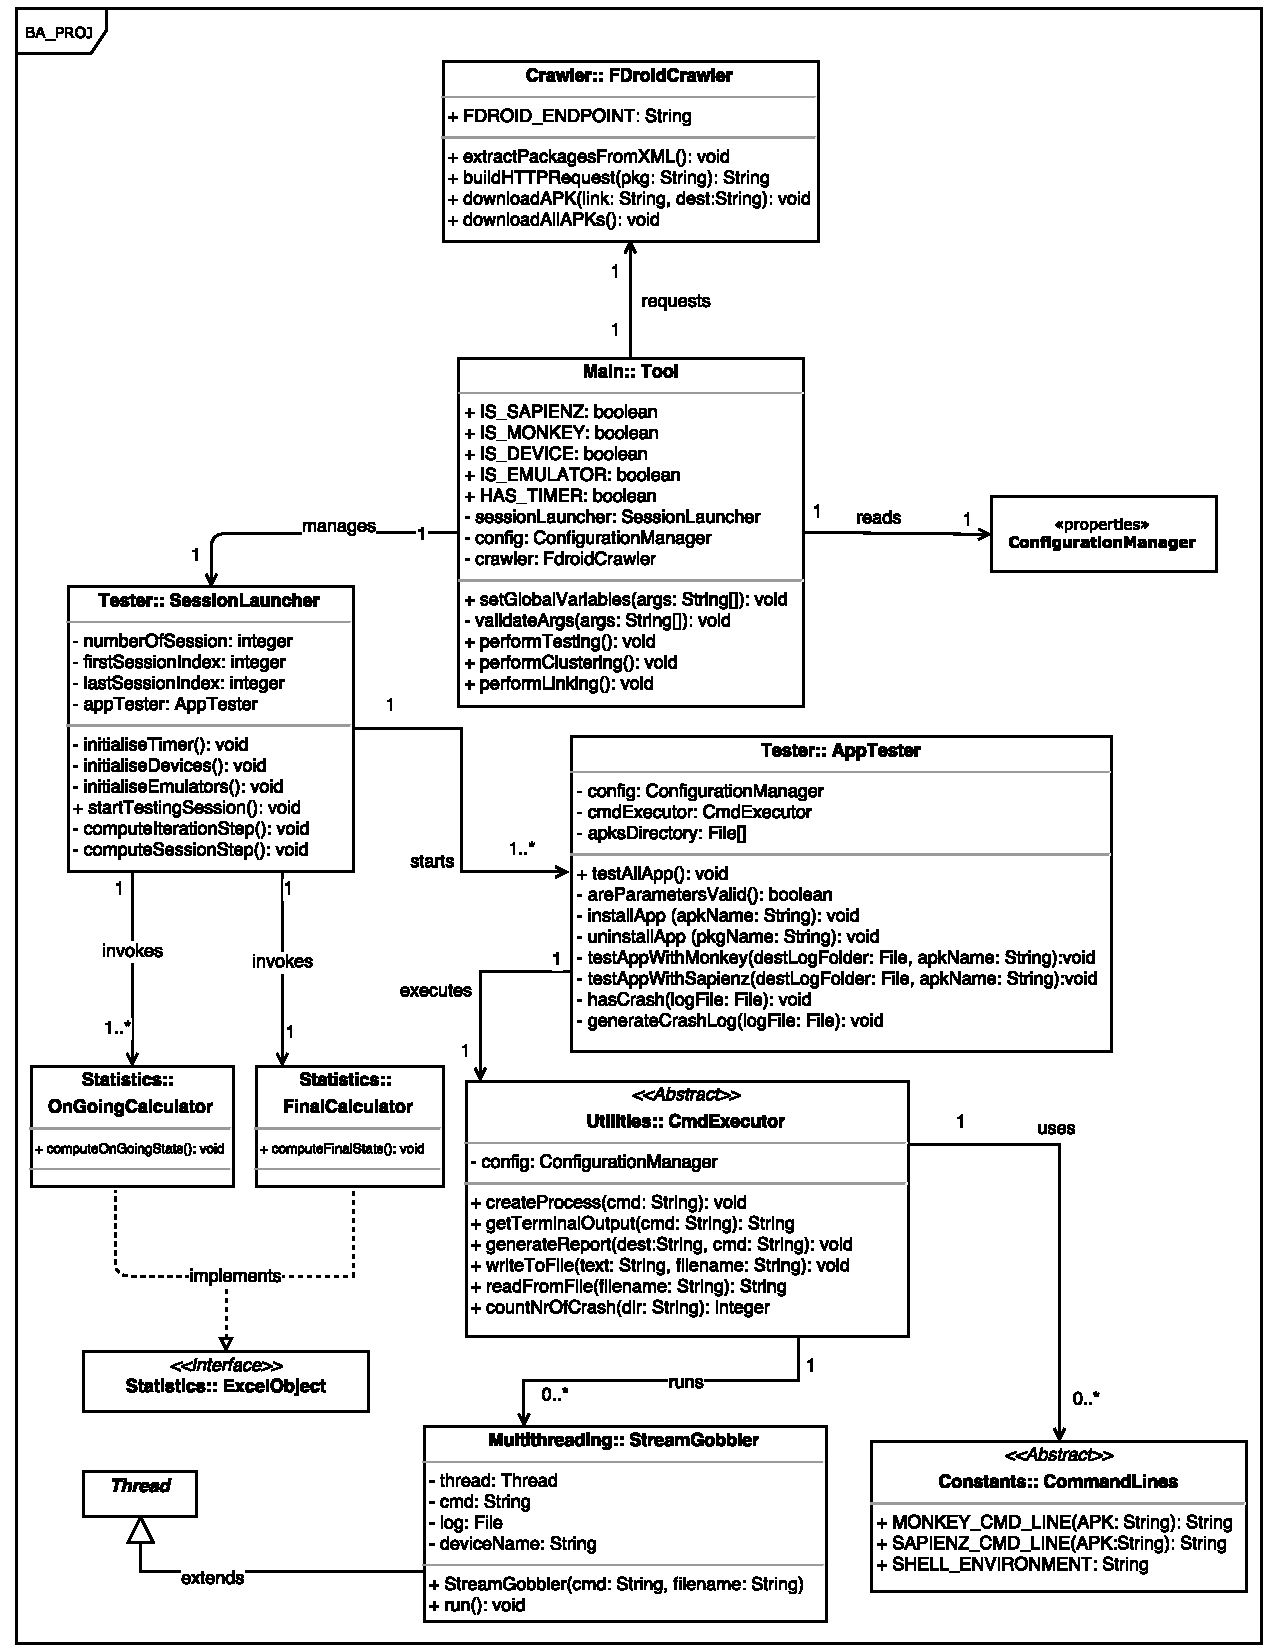
\includegraphics[width=\columnwidth]{diagrams/testing.pdf} 
\caption{Class Diagram of the testing part of the tool }
\label{testing}
\vspace{-3mm} 
\end{figure}


\begin{figure}[t]
\centering 
%	\vspace{-1.5mm} 
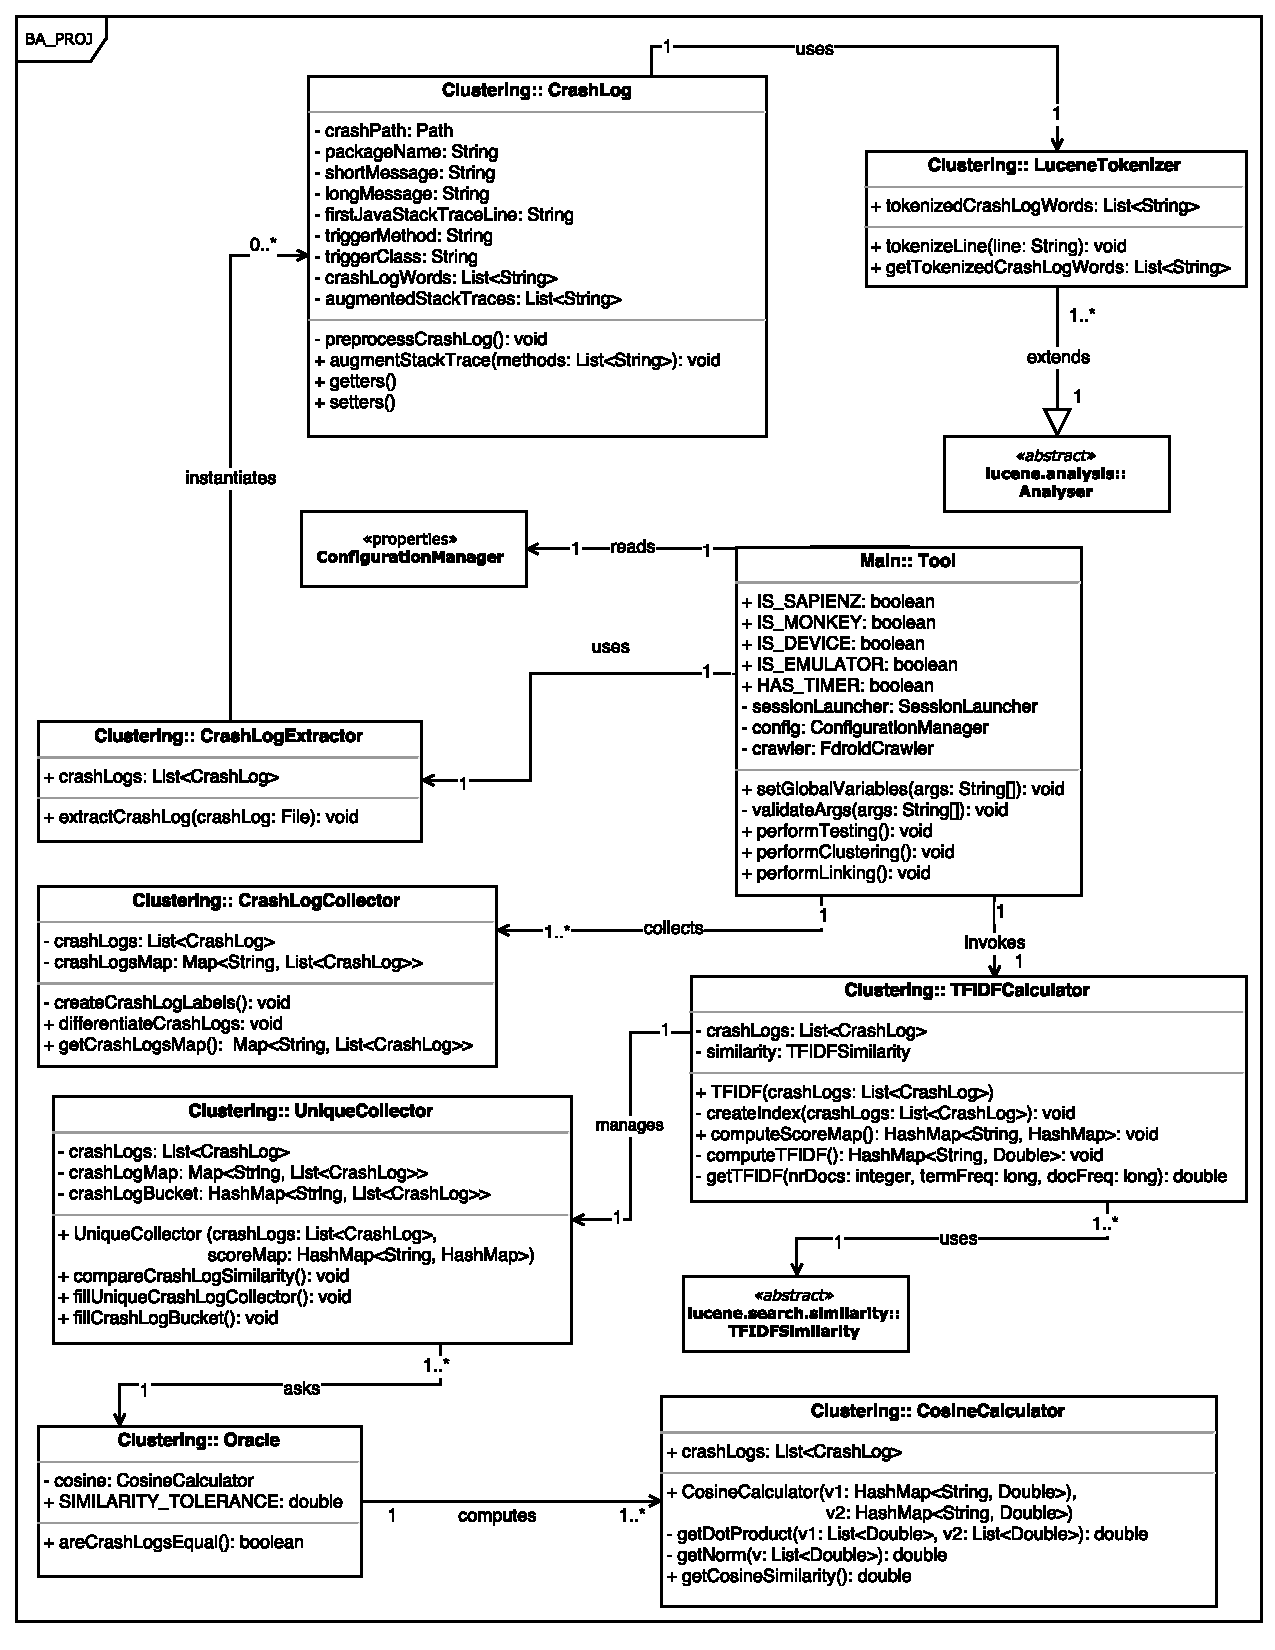
\includegraphics[width=\columnwidth]{diagrams/clustering.pdf} 
\caption{Class Diagram of the clustering part of the tool }
\label{clustering}
\vspace{-3mm} 
\end{figure}


\begin{figure}[t]
\centering 
%	\vspace{-1.5mm} 
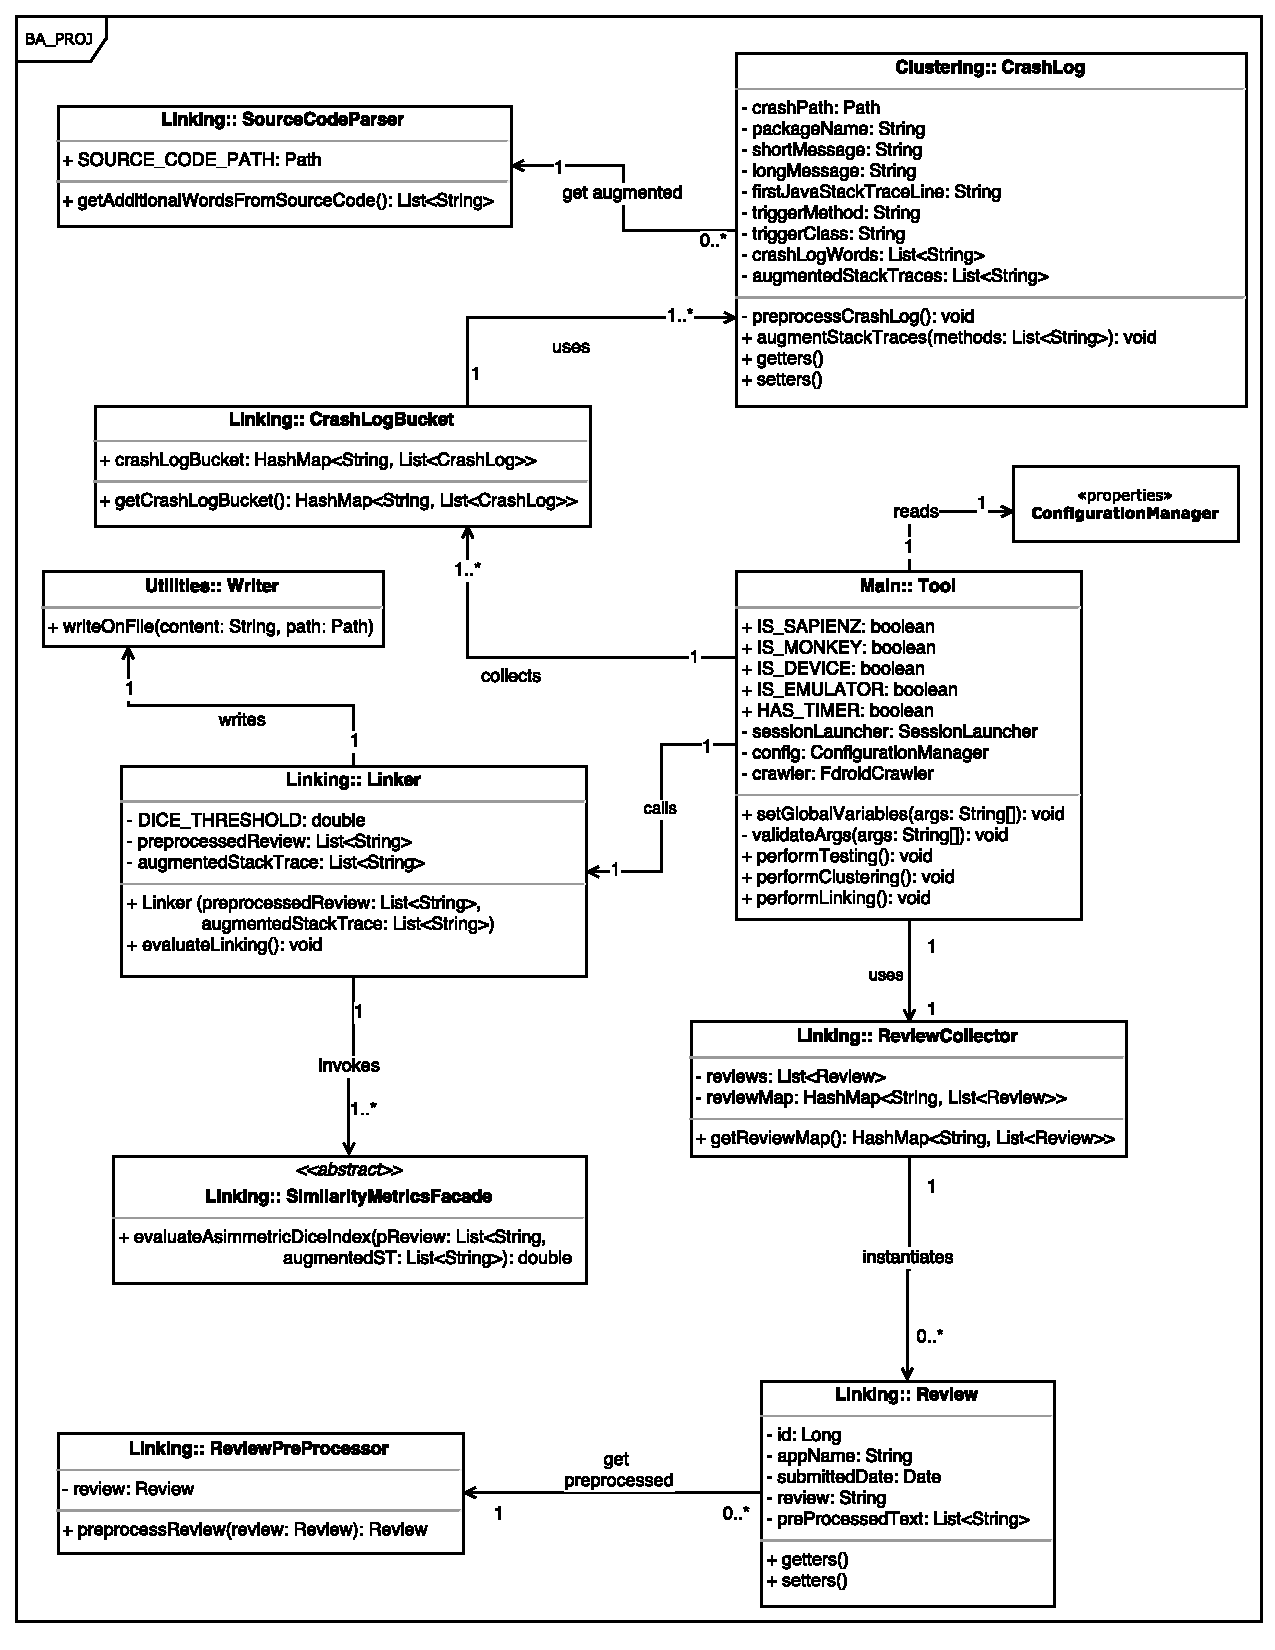
\includegraphics[width=\columnwidth]{diagrams/linking.pdf} 
\caption{Class Diagram of the linking part of the tool }
\label{linking}
\vspace{-3mm} 
\end{figure}

\chapter{Results and Discussion}

\chapter{Conclusions and Future Work}




\backmatter
%alpha
\bibliographystyle{abbrv}
\bibliography{biblio}

\end{document}


% ampliare sezione review Related Work
%RQ2 -> risposta precisione table II paper
%RQ3 -> IC, IR, IT -> fare leva sulle review per aumentare l'efficacia del testing 





